\chapter{基于密集型自底向上网络的视频片段检索方法}

在本章,我们主要解决视频片段检索任务。具体来说,给定一个查询(如:自然语句或者视频片段)和一段未裁剪的视频序列,模型需要在视频序列中定位出和查询内容相匹配的片段。目前,主流的视频片段检索方法可以分为两大类:(1)自顶向下(Top-down)的方法:它们先将整个视频序列切分为若干候选片段,然后对每个候选片段进行分类和回归。分类主要是计算候选片段与查询的相似度,回归主要是微调片段的位置。(2)自底向上(Bottom-up)的方法:先将视频序列和查询进行特征融合,然后对融合后的特征序列中的每一帧预测其属于视频序列定位边界的概率(起始时刻和终止时刻)。然后这两类方法都各自具有明显的缺点:自顶向下的方法需要人为地预先设定许多切分的规则(如:候选片段的大小、候选片段的数量等)同时定位速度也较慢,而自底向上的方法的性能还低于自顶向上的方法。在本章,我们重点分析了目前的自底向上方法的设计缺陷,提出了一种全新的密集型自底向上框架。我们将位于起始时刻和终止时刻之间的每一帧都看成是正样本,每一个正样本帧都回归一个独特的离定位边界的距离。同时为了更好的适应密集型自底向上的框架,我们还提出了一种基于图结构的特征金字塔网络,来强化目前的骨干网络(backbone)。我们先将多尺度的特征帧映射到同一个语义空间中,然后利用图卷积学习到语义空间中不同特征的内在联系。我们在常用的四个视频片段检索数据集(TACoS~\cite{regneri2013grounding}、Charades-STA~\cite{gao2017tall}、ActivityNet Captions~\cite{krishna2017dense}、Activity VRL~\cite{feng2018video})中验证了我们方法的有效性,我们提出的密集型自底向上网络不仅可以在性能上超过目前所有的方法,同时可以保持和其他自底向上的模型相同的定位速度。


\section{问题描述}

基于查询的视频片段检索(Query-based Video Localization, QBVL)是视频场景理解领域一个重要的研究问题。它不仅仅需要准确地把握检索内容的语义信息,同时需要对视频内容有正确的理解。随着大规模视频数据集的出现和视频特征学习的发展,目前主要有两种视频片段检索任务:(1)第一种是基于语句的视频片段检索,即查询内容是一个自然语言描述语句(如图~\ref{ch6:fig:qbvl}(a))。(2)第二种是基于视频片段的视频片段检索,即查询内容是包含一个动作的短视频片段(如图~\ref{ch6:fig:qbvl}(b))。这两种视频片段检索任务拥有同样的目标:在视频序列中定位出两个边界时刻(即起始时刻和终止时刻),使得从起始时刻到终止时刻之间的视频片段内容刚和和查询内容一致。视频片段检索任务也是许多重要的视频应用的技术基础,例如:基于内容的精彩片段检索、行人重识别等。

\begin{figure}[htbp]
    \centering
    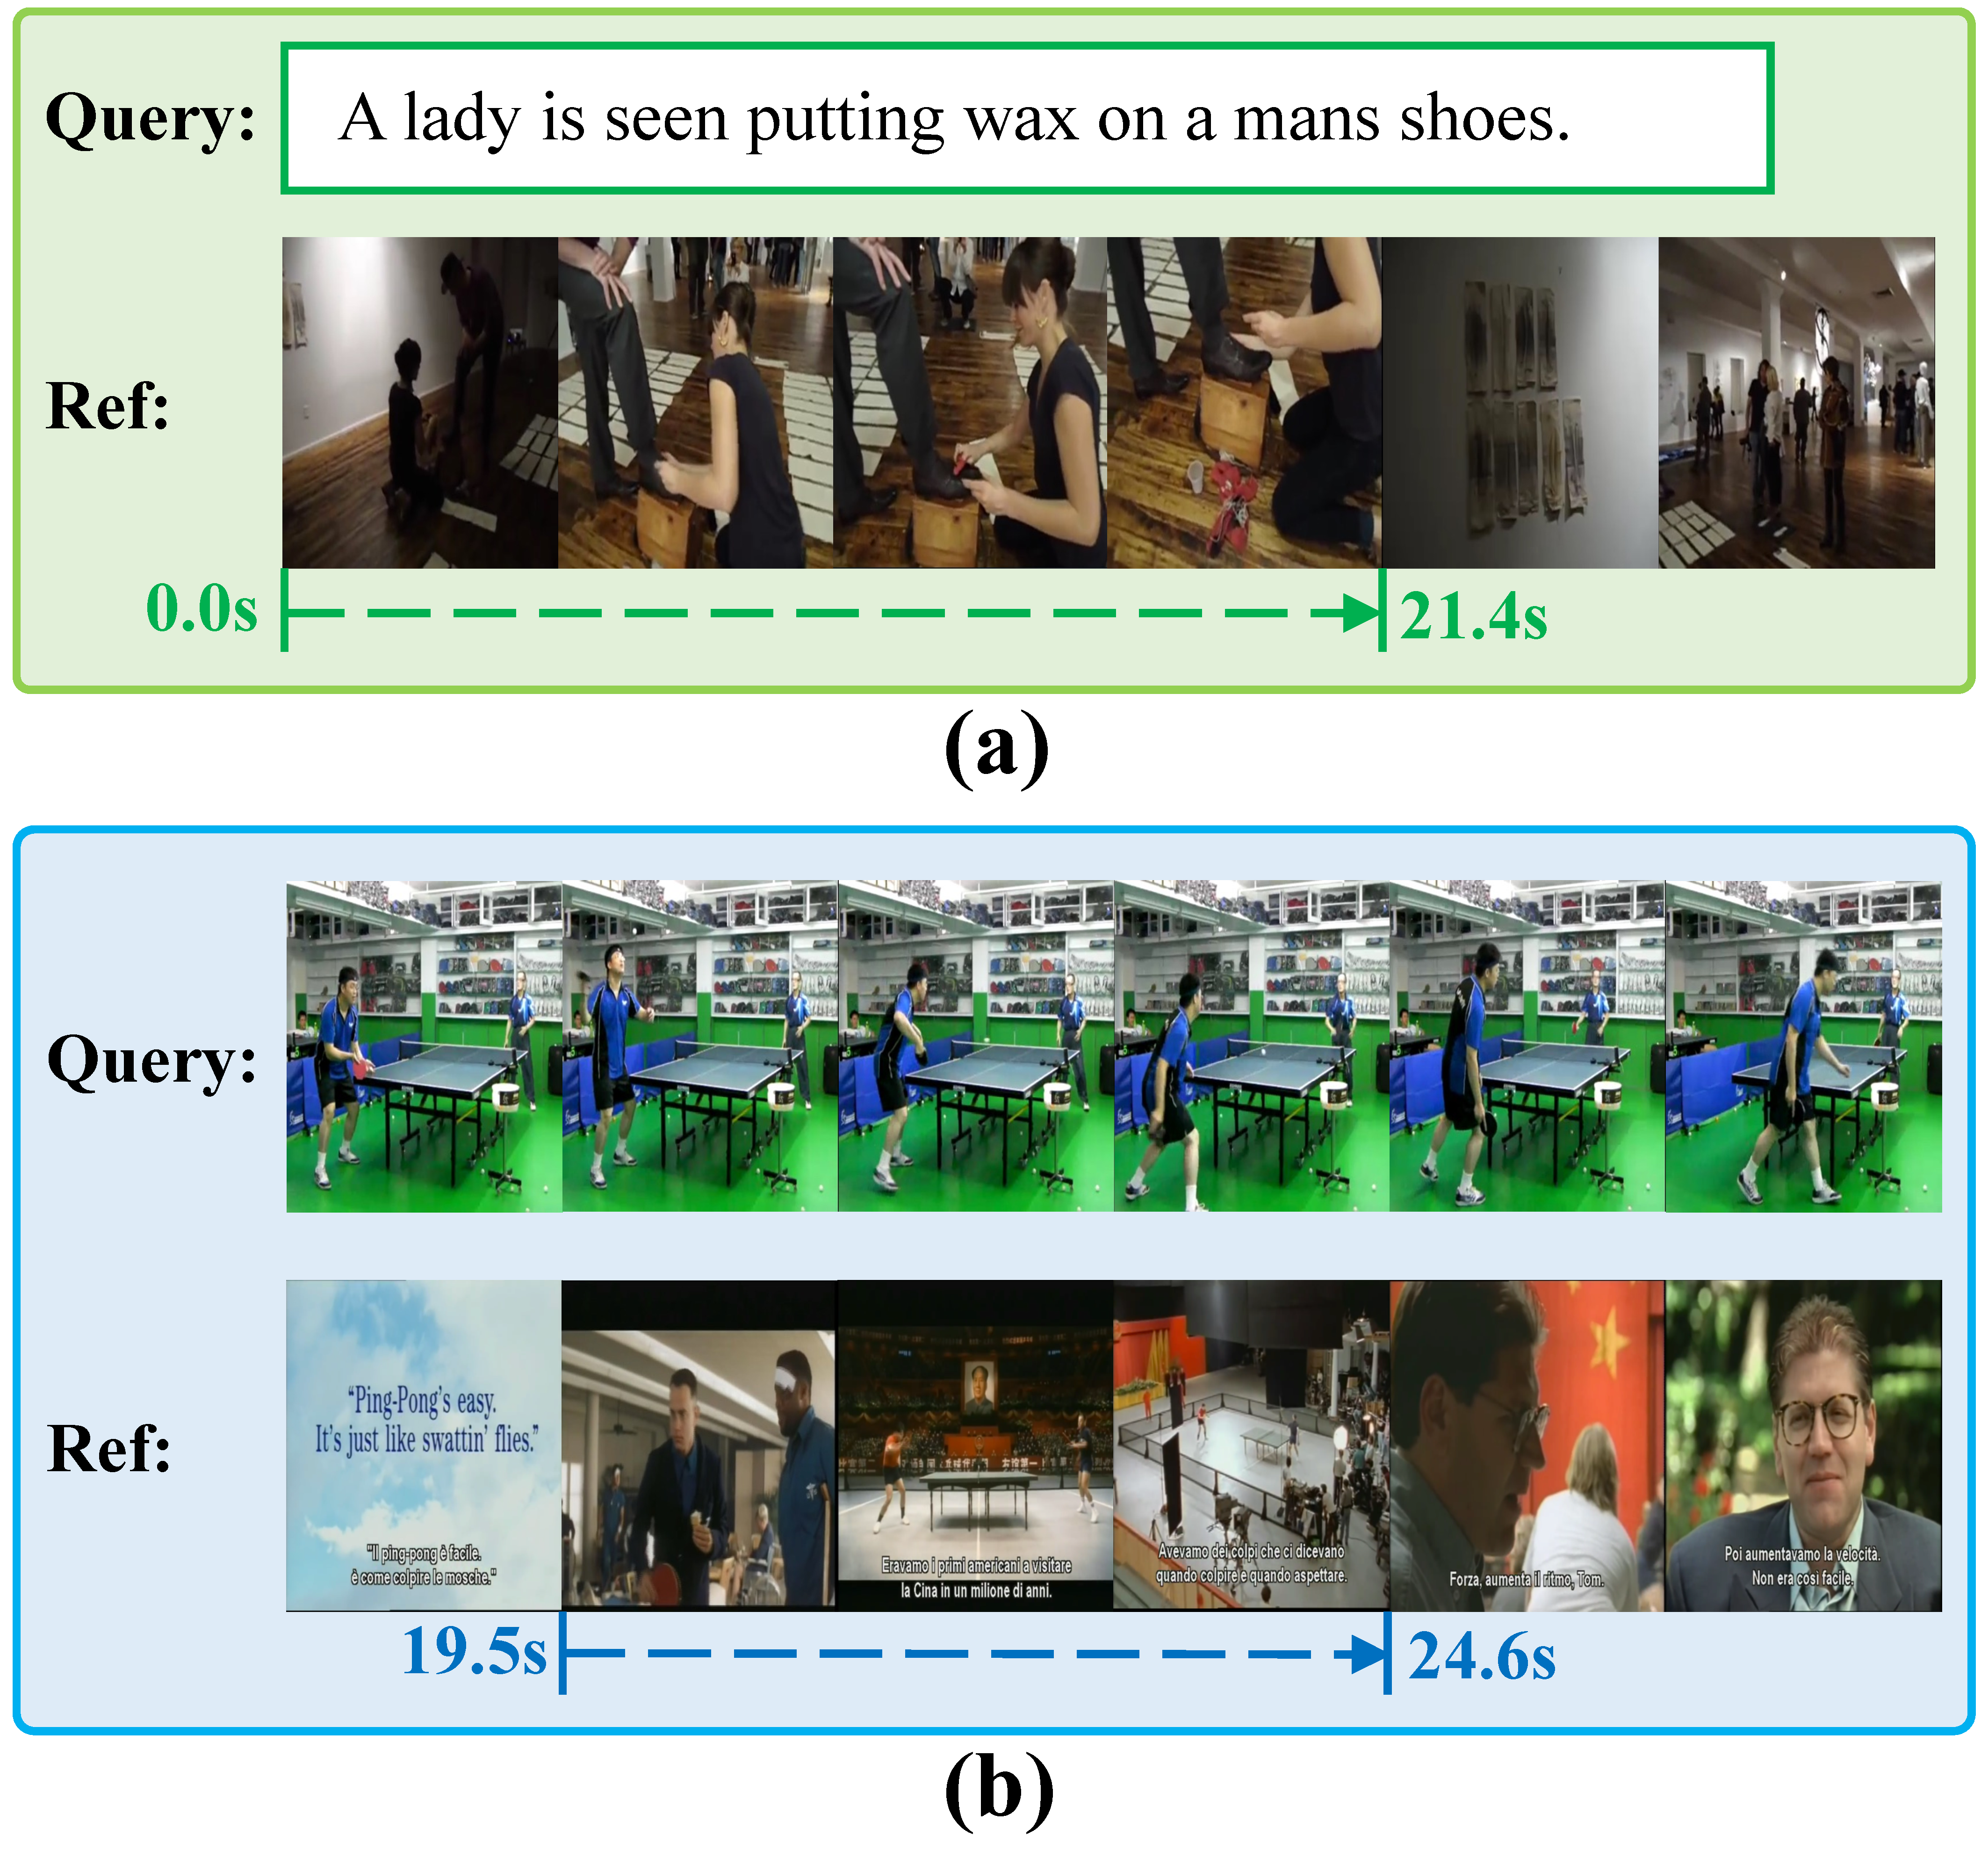
\includegraphics[width=0.7\linewidth]{chapter6/res/qbvl.pdf}
    \caption{两种视频片段检索任务}
    \label{ch6:fig:qbvl}
\end{figure}

到目前为止,绝大多数的视频片段检索方法都属于\textbf{自顶向下}框架:它们将视频序列切分为众多的候选视频片段,然后对每个候选片段进行分类和回归任务。具体来说,这种自顶向下的框架又可以分为两类:(1)滑窗型~\cite{gao2017tall,anne2017localizing,liu2018attentive,liu2018cross,ge2019mac,chen2019semantic,xu2019multilevel,zhang2019exploiting}:它们预先定义一系列不同大小的滑窗,然后通过滑窗密集地将视频“显式”地切分成若干候选视频片段,最后对查询和候选片段分别提取特征。这样,基于查询的视频片段检索问题就转变为一个简单的相似度匹配问题。但是这类方法忽略了视频中周围其他视频帧的内在联系,这些周围帧往往对视频理解有着巨大的帮助~\cite{wu2019long}。(2)锚框型~\cite{chen2018temporally,zhang2019man}:它们不像滑窗型直接将视频预先切分,而是在每个视频帧上都定义若干锚框,然后对每个锚框内的视频进行分类和预测。为了充分利用周围的视频帧,它们通常用递归神经网络将所有的视频帧进行串接。这类方法可以看成是基于锚框型的目标检测方法~\cite{ren2015faster}在视频领域的拓展。

尽管这些自顶向下的模型(包括滑窗型和锚框型)可以在多个数据集上达到目前最好的性能,但是这类方法本质上仍然许多一些不可避免的缺点:(1)最终的实验结果受预先定义的规则影响较大(如滑窗或锚框的大小、数量等);(2)为了尽可能的提高召回率,模型必须增大滑窗或锚框数量,导致计算量增大、定位速度慢。


\begin{figure}[htbp]
    \centering
    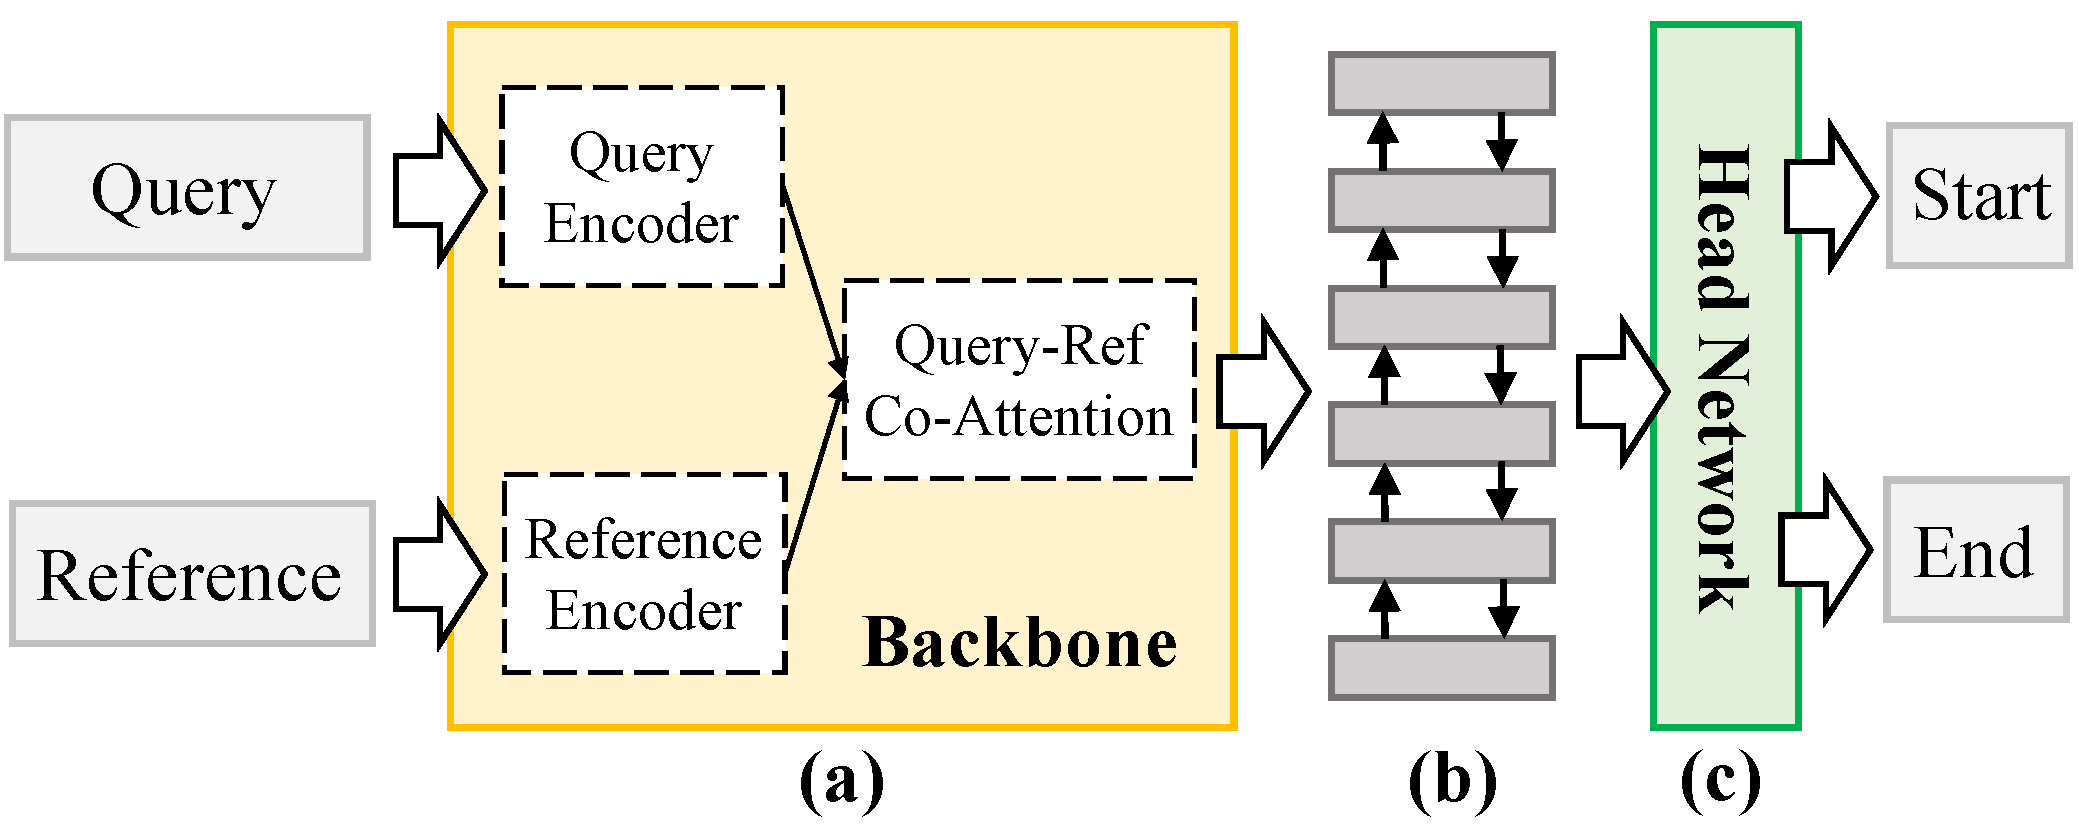
\includegraphics[width=0.7\linewidth]{chapter6/res/sparse_bu.pdf}
    \caption{典型的稀疏型自底向上视频片段检索模型}
    \label{ch6:fig:sparse_bu}
\end{figure}


为了消除这些缺点,一些视频片段检索方法~\cite{chen2019localizing,yuan2019find,feng2018video}开始借鉴现有的阅读理解(Reading Comprehension)的模型\cite{xiong2017dynamic,xiong2018dcn+,yu2018qanet},用一种\textbf{稀疏型自底向上}的网络直接预测两个边界的概率。如图~\ref{ch6:fig:sparse_bu}所示,一个典型的稀疏型自底向上模型主要包含两个组成部分:骨干网络(图~\ref{ch6:fig:sparse_bu}(a))和头网络(图~\ref{ch6:fig:sparse_bu}(c))。骨干网络通常会使用协同注意力机制(co-attention)来融合查询内容的特征和每个视频帧的特征,它的输出是融合后的特征序列(图~\ref{ch6:fig:sparse_bu}(b))。为了后续的头网络能对视频序列的每一帧直接预测边界概率,融合后的特征序列往往需要保持和输入视频相同的长度。尽管这种稀疏型自底向上的方法可以避免自顶向下方法的缺点,但是它们的性能却仍然低于自顶向下方法,尤其是对于长视频(如:数据集TACoS)。我们认为自底向上方法的性能低于自顶向下方法的主要原因来自于目前骨干网络和头网络的不合理设计:

\textbf{骨干网络}(Backbone Network):对于骨干网络的设计,目前的稀疏型自底向上模型的骨干网络主要有两个缺点:(1)每个视频包含丰富的场景变化,即不同的视频场景分布在视频的不同位置。因此,理解视频不同场景的变化以及场景之间的关系对于充分理解视频内容至关重要。然后,目前的方法通常使用递归神经网络RNN来编码每一帧的特征(帧级别),而忽略了场景级别的关系。(2)为了方便头网络的预测,骨干网络需要让融合后的特征序列保持和原始视频相同的分辨率,这容易导致模型只编码局部的语义信息,而忽略全局的语义信息~\cite{chen2018encoder,lin2017feature}。

\textbf{头网络}(Head Network):对于头网络的设计,目前的稀疏型自底向上模型的头网络主要有三个缺点:(1)两个边界时刻(起始时刻和终止时刻)的预测是相互独立的,即模型预测边界时忽略了两个边界内部视频内容的一致性。如图~\ref{ch6:fig:headnetwork_motivation}(a),在时刻B和时刻D时的视频有非常相似的场景内容,因此,模型很容易将结果预测为(A$\to$D),即使在时刻(B$\to$C)之间有明显的场景内容变化。(2)训练过程时,正样本和负样本的数量极度不均。因为视频的长度通常较长(如:数据集TACoS中每个视频的平均长度为9000帧),而只有两帧为证样本(即起始时刻帧和终止时刻帧,如图~\ref{ch6:fig:headnetwork_motivation}(b))。(3)没有查询的约束,对视频中发生动作的边界进行预测本身仍是目前未解决的开放性难题~\cite{shou2018online}。因为它一方面需要判断每个视频帧内容和查询内容是否相关,另一方面也需要判断该视频帧是否为动作边界。

\begin{figure}[tbp]
    \centering
    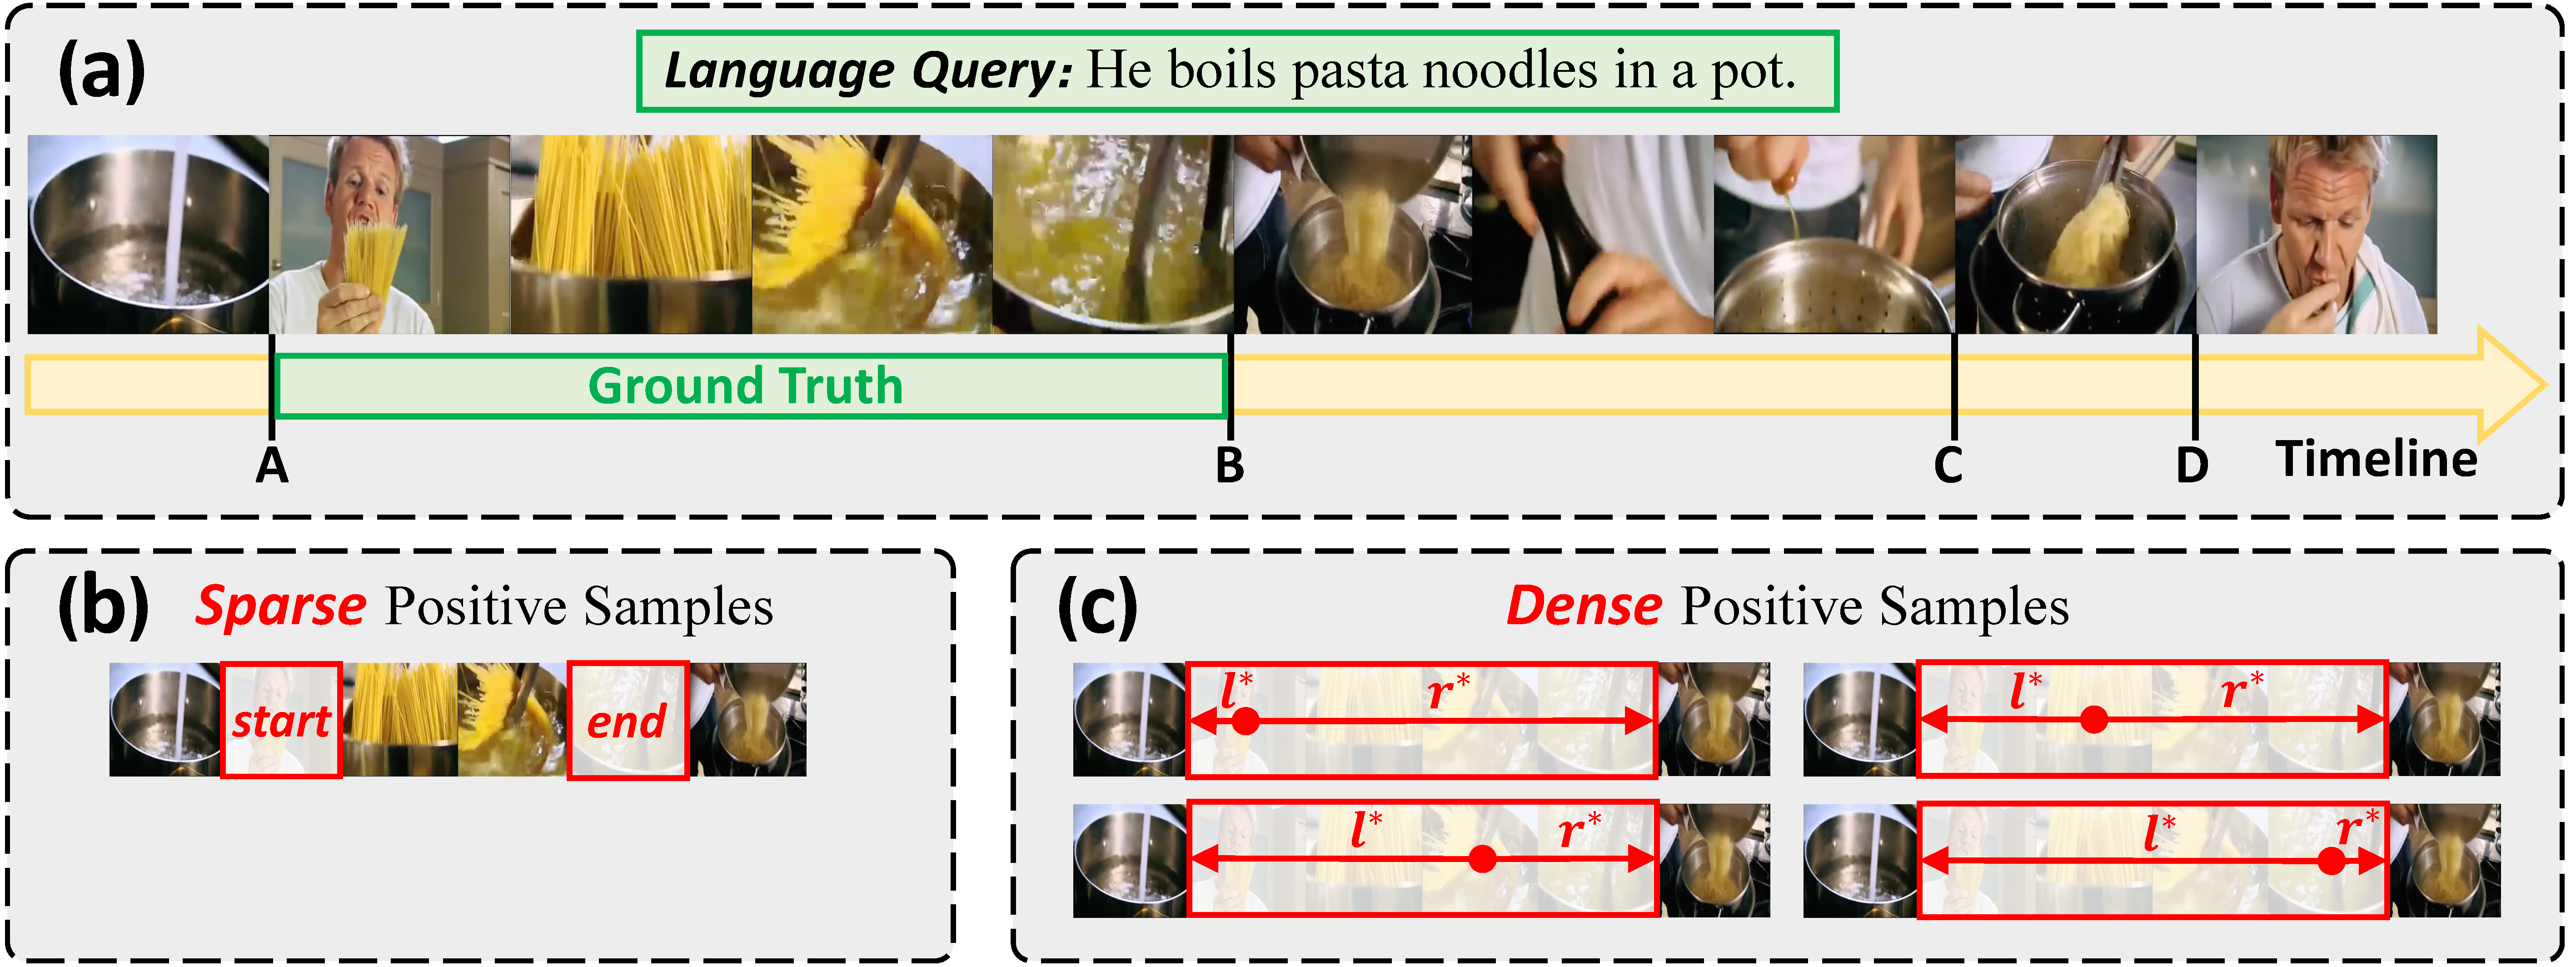
\includegraphics[width=0.95\linewidth]{chapter6/res/headnetwork_motivation.pdf}
    \caption{一个基于语句的视频片段检索示例}
    \label{ch6:fig:headnetwork_motivation}
\end{figure}


在本章,我们针对稀疏型自底向上模型的缺点,提出了一种全新的密集型自底向上网络:基于图特征金字塔的密集型预测(Graph-FPN with Dense Prediction, GDP)。对于骨干网络,GDP引入一个图特征金字塔层来增强骨干网络的输出(图~\ref{ch6:fig:sparse_bu}(b))。GDP首先构建一个金字塔多尺度特征,然后将不同尺度的特征序列映射到一个高语义的场景空间中,然后利用图卷积对场景空间中的节点进行特征融合。图卷积不仅可以充分利用不同语义场景之间的内在联系,同时可以消除不同尺度下特征的语义差。最后这些场景空间的特征合成为新的特征序列。对于头网络,我们将起始时刻到终止时刻之间的每一帧都看成是正样本。对于每个正样本,GDP包含一个回归网络来预测从当前帧到两个边界时刻各自的距离。这样的设计一方面可以缓解训练过程中正负样本极度不均的问题,另一方面由于两个边界预测来自于同一个特征,可以避免陷入独立预测的局部最优。同时,GDP包含一个置信网络来预测当前帧与查询的关联度,可以将边界帧预测任务分离成关联度判断和边界回归两个任务,减少任务难度。


我们在常用的四个视频片段检索数据集(TACoS~\cite{regneri2013grounding}、Charades-STA~\cite{gao2017tall}、ActivityNet Captions~\cite{krishna2017dense}、Activity VRL~\cite{feng2018video})中验证了GDP的有效性。GDP在多个指标下都超过了目前所有的自顶向下的方法,同时保持了自底向上方法的定位速度。

\section{基于图特征金字塔的密集型预测}

给定一个视频序列$\mathcal{V}$和查询$\mathcal{Q}$,基于查询的视频片段检索任务(QBVL)需要预测出两个边界时刻($t_s, t_e$),满足从$t_s$到$t_e$之间的视频片段内容与查询内容刚好一致。在本节我们将介绍GDP模型的每一个组合部分~\ref{ch6:fig:dense_bu},包括一个骨干网络(a)、一个图特征金字塔层(b)和一个密集型头网络(c),然后我们再介绍GDP的训练和测试过程。

\begin{figure}[htbp]
    \centering
    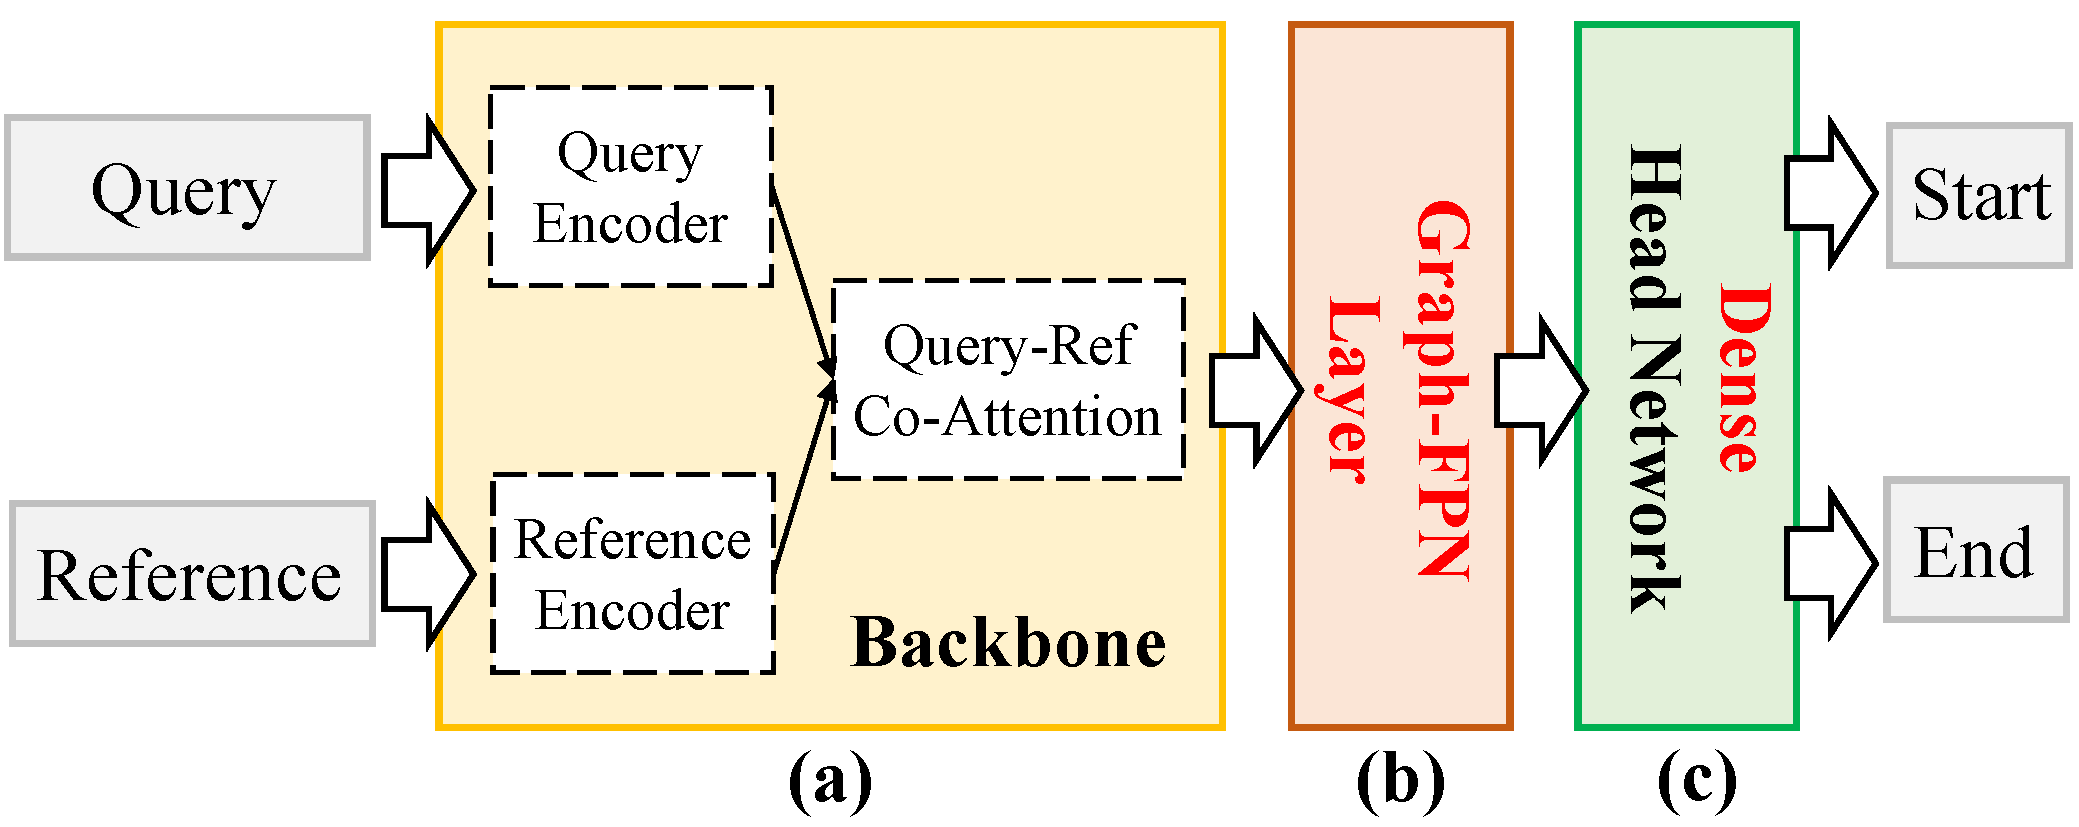
\includegraphics[width=0.7\linewidth]{chapter6/res/dense_bu.pdf}
    \caption{典型的稀疏型自底向上视频片段检索模型}
    \label{ch6:fig:dense_bu}
\end{figure}

\subsection{骨干网络}
GDP的骨干网络使用QANet~\cite{yu2018qanet}来融合查询和视频的特征。如图~\ref{ch6:fig:qanet}所示,QANet共有两个输入:查询特征$\bm{Q} = \{\bm{q}_n\}^N_{n=1}$和视频序列特征$\bm{V}=\{\bm{v}_i\}^T_{i=1}$,其中$N$和$T$分别表示查询和视频的长度。具体来说,QANet包含四个主要部分:

\textbf{查询特征编码器}:查询特征编码器包含多个特征编码层(如图~\ref{ch6:fig:qanet}(b)),每个特征编码层有卷积层、层归一化层、自注意力层和全连接层组成。查询特征编码器的输出是$\bm{\tilde{Q}}=\{\bm{\tilde{q}}_n\}^N_{n=1}$。

\textbf{视频特征编码器}:视频特征编码器的结构和查询特征编码器完全相同,即由多个特征编码层组成(如图~\ref{ch6:fig:qanet}(b)),并且视频特征编码器的输出是$\bm{\tilde{V}} = \{\bm{\tilde{v}}_i\}^T_{i=1}$。


\textbf{查询-视频协同注意力层}:它包含一个协同注意力机制来融合查询特征$\bm{\tilde{Q}}=\{\bm{\tilde{q}}_n\}^N_{n=1}$和视频特征$\bm{\tilde{V}} = \{\bm{\tilde{v}}_i\}^T_{i=1}$。具体来说,它先计算一个相似矩阵$\bm{S}\in\mathbb{R}^{T\times N}$,其中每个元素$\bm{S}_{ij}$表示$\bm{\tilde{v}}_i$和$\bm{\tilde{q}}_j$之间的相似度。然后可以得到两个加权特征:
\begin{equation}
  \bm{A} = \bar{\bm{S}} \cdot \tilde{\bm{Q}}, \quad \bm{B} = \bar{\bm{S}} \cdot \bar{\bar{\bm{S}}}^T \cdot \tilde{\bm{V}},
\end{equation}
其中$\bar{\bm{S}}$和$\bar{\bar{\bm{S}}}$分别是对$S$按行和按列进行归一化。


\begin{figure}[tbp]
    \centering
    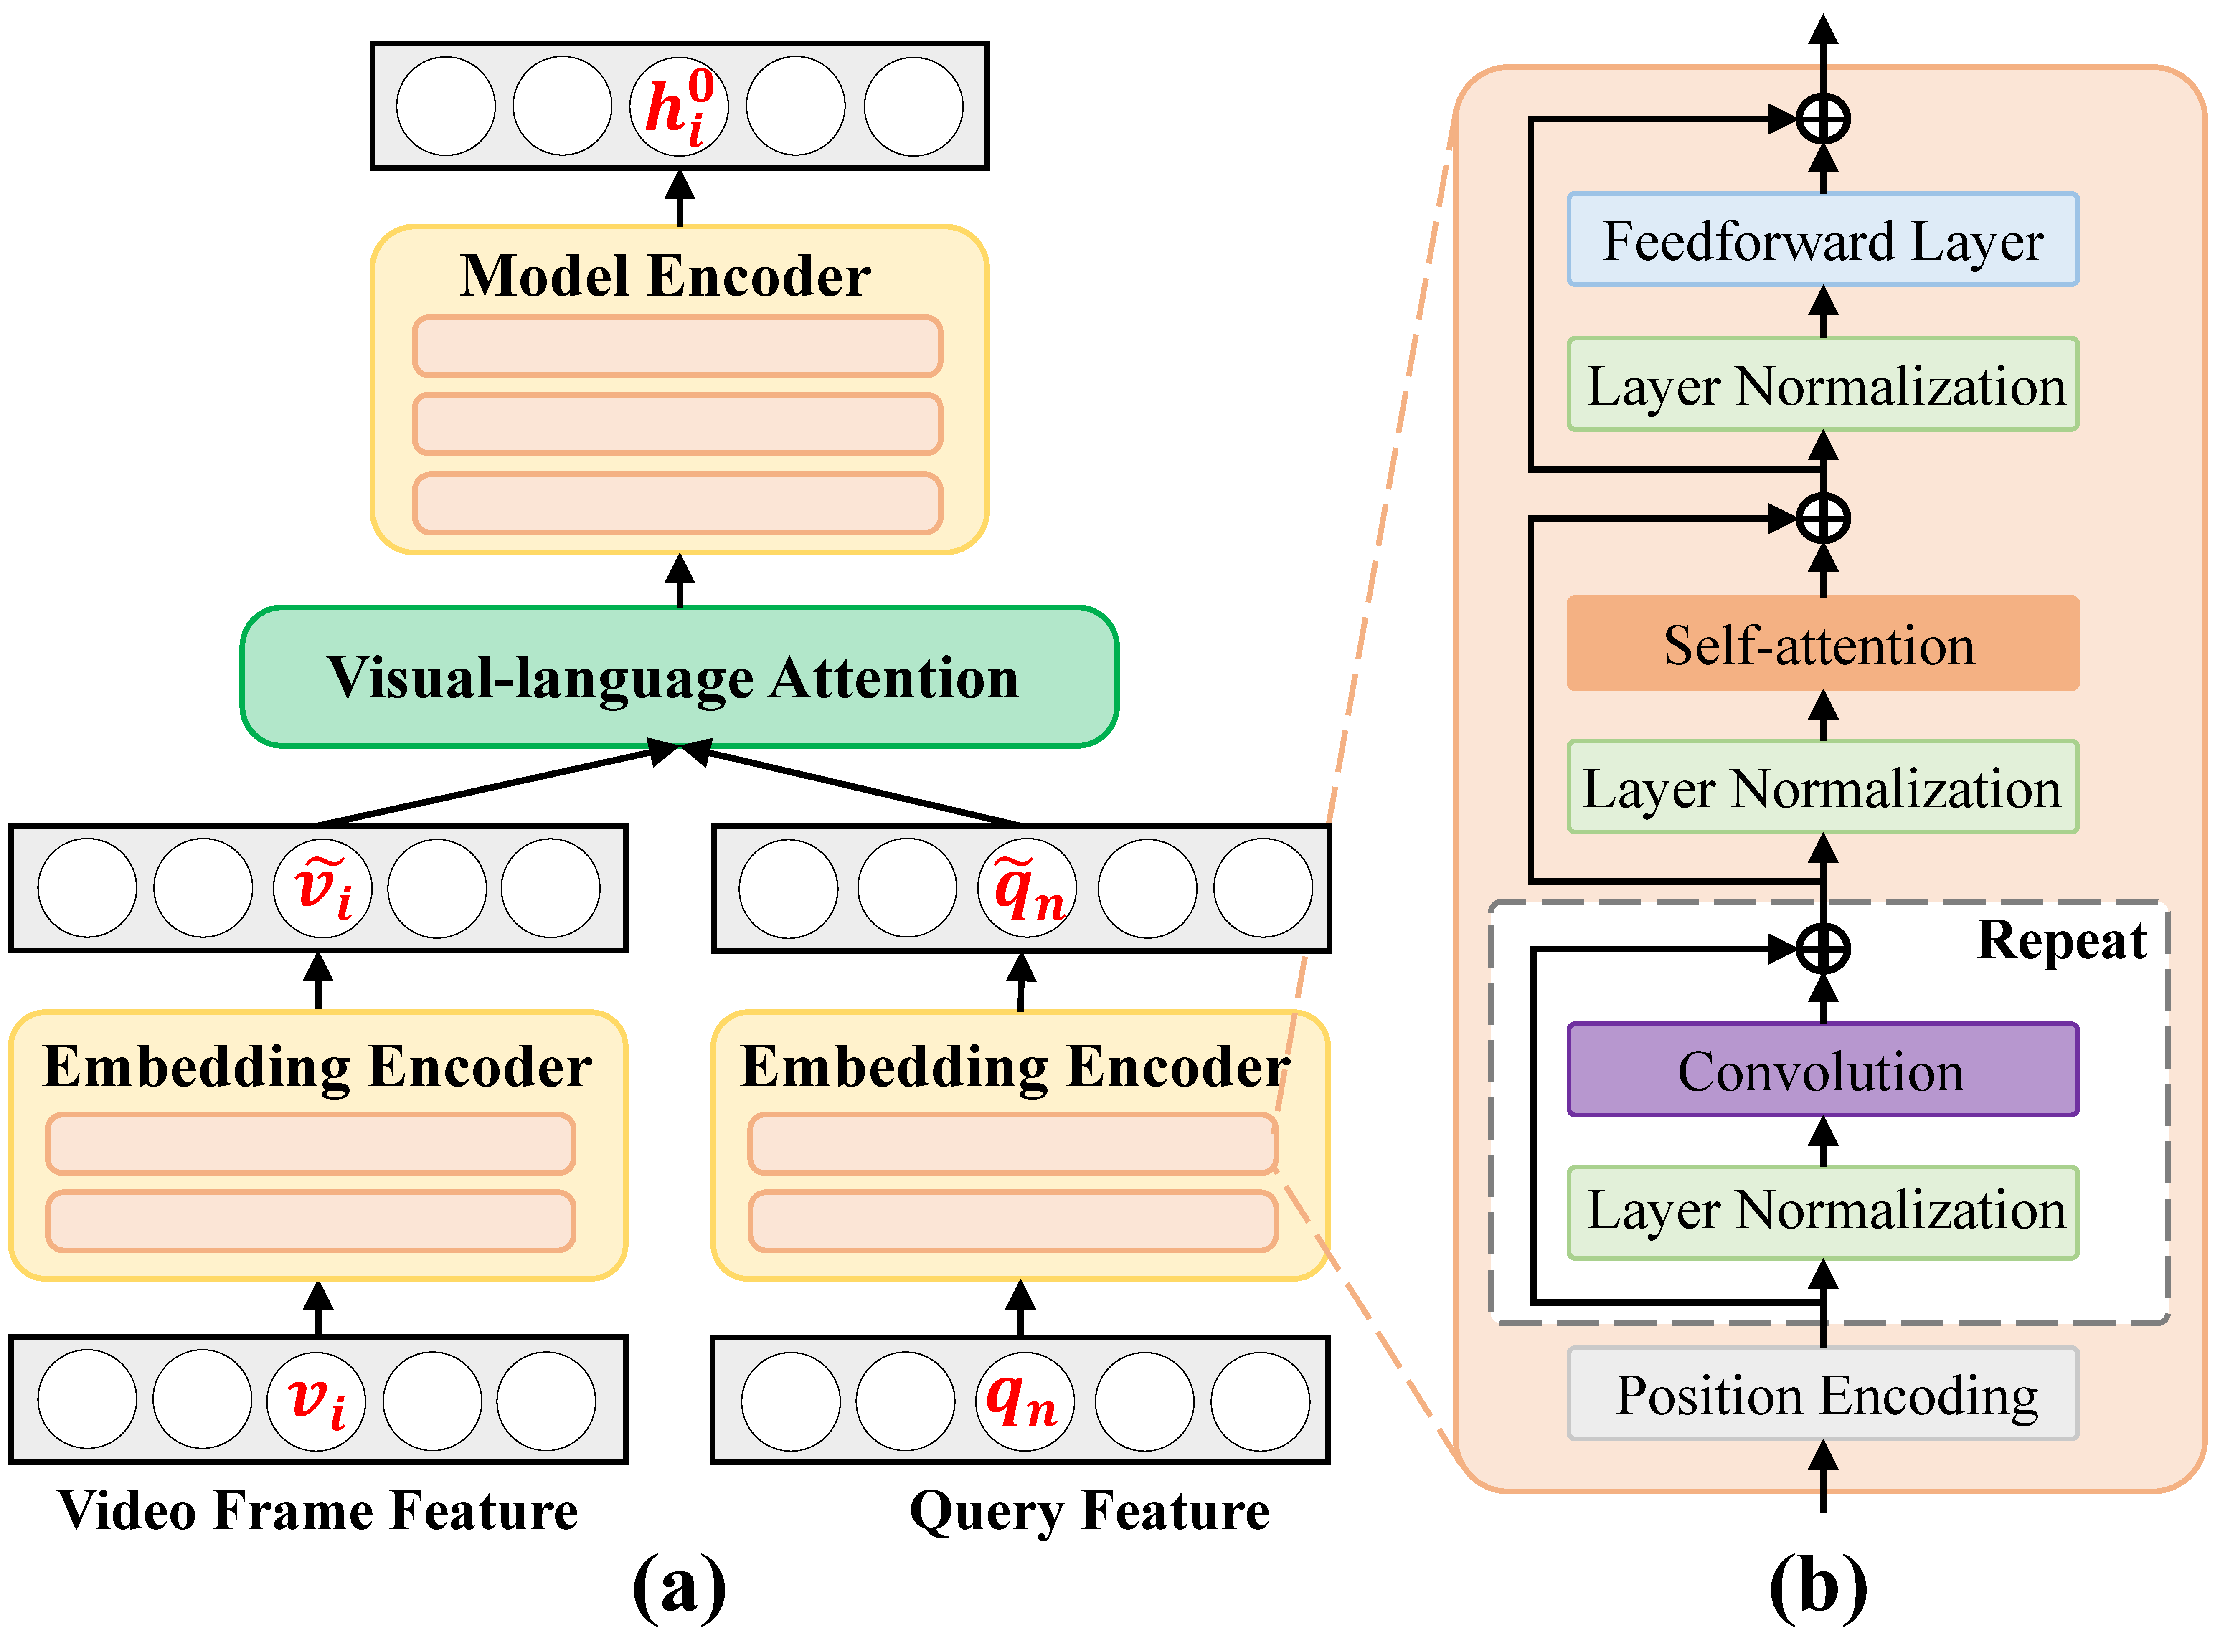
\includegraphics[width=0.7\linewidth]{chapter6/res/qanet.pdf}
    \caption{骨干网络QANet}
    \label{ch6:fig:qanet}
\end{figure}


\textbf{融合特征编码器}:给定两个注意力权重$\bm{A}$和$\bm{B}$,融合特征编码器开始对融合后的特征进行编码。融合特征编码器同样由多层特征编码层(图~\ref{ch6:fig:qanet}(b))组成。融合特征编码器的输入是一个特征序列,它的第$i$个特征为$[\bm{v}_i, \bm{a}_i, \bm{v}_i\odot \bm{a}_i, \bm{v}_i\odot \bm{b}_i]$,其中$\bm{a}_i$和$\bm{b}_i$分别是矩阵$\bm{A}$和$\bm{B}$的第$i$行,$\odot$是元素积,$[,]$是向量连接符。融合特征编码器的输出为$\bm{H}_0=\{\bm{h}^0_i\}^T_{i=1}$,$\bm{H}_0 \in \mathbb{R}^{T\times D}$,其中每个特征$\bm{h}^0_i \in \mathbb{R}^D$都包含了查询信息。现有的稀疏型自底向上模型通常直接将$\bm{H}_0$作为头网络的输入,与现有模型不同,GDP包含一个图特征金字塔层对特征$\bm{H}_0$进行增强。值得注意的是,GDP模型对任意的骨干网络都可以无缝的兼容。


\subsection{图特征金字塔层}
如图~\ref{ch6:fig:graph_fpn},图特征金字塔层主要包含四个步骤来增强骨干网络输出$\bm{H}_0$:

\textbf{特征金字塔构建}:给定$\bm{H}_0$,我们首先通过逐渐减少特征序列长度来构建特征金字塔$\{\bm{H}_1 \in \mathbb{R}^{T_1\times D}, \bm{H}_2 \in \mathbb{R}^{T_2\times D}, \bm{H}_3 \in \mathbb{R}^{T_3\times D}\}$,其中$T_{i+1} = T_i/2$。我们同样使用相同的多个特征编码层(如图~\ref{ch6:fig:qanet}(b))和一个额外的步长为2的卷积层将特征$\bm{H}_i$转换为$\bm{H}_{i+1}$。

\textbf{帧空间到场景空间}:在得到多个尺度的特征$\{\bm{H}_1, \bm{H}_2, \bm{H}_3\}$之后,我们将这些特征从原始的帧空间映射到场景空间。以$\bm{H}_2 = \{\bm{h}^2_i\}^{T_2}_{i=1}$为例子,我们希望得到一系列场景空间特征$\bm{X}_2 = f_2(\bm{H}_2) \in \mathbb{R}^{N_2\times D}$,其中$N_2$表示场景空间在该尺度的节点数量,映射函数$f_2(\cdot)$是对原始输入特征的线性组合:
\begin{equation} \label{ch6:eq:eq_2}
    \bm{x}^2_i = \bm{c}^2_i \bm{H}_2 = \sum\nolimits_j c^2_{ij}\bm{h}^2_j,
\end{equation}
其中$\bm{C}_2 = [\bm{c}^2_1, ..., \bm{c}^2_{N_2}]$,$\bm{C}_2 \in \mathbb{R}^{N_2\times T_2}$。$\bm{C}_2$由$\bm{H}_2$经过一个$1\times1$卷积得到。相似地,我们可以通过$\bm{H}_1$、$\bm{H}_3$得到$\bm{X}_1 \in \mathbb{R}^{N_1\times D}$、$\bm{X}_3 \in \mathbb{R}^{N_3\times D}$。


\textbf{场景空间图卷积}:当把不同尺度的特征都从帧空间映射到场景空间之后,我们使用图卷积~\cite{kipf2017semi}里编码不同场景间的关系。具体来说,我们将所有的$N_{total}$节点($N_{total} = N_1 + N_2 + N_3$)看成一个全连接图,然后利用图卷积进行参数更新:
\begin{equation}
    \bm{Y} = ((\bm{I}-\bm{A}_{adj})\bm{X})\bm{W},
\end{equation}
其中,$\bm{X} = [\bm{X}_1; \bm{X}_2; \bm{X}_3] \in \mathbb{R}^{N_{total}\times D}$是场景空间所有节点特征的集合,[;]表示矩阵中行连接符,$\bm{W}\in \mathbb{R}^{D\times D}$是映射矩阵,$\bm{A}_{adj}$是可学习的邻接矩阵,大小为$N_{total}\times N_{total}$,$\bm{I}$是单位矩阵。


\textbf{场景空间到帧空间}:给定场景空间特征$\bm{Y} = [\bm{Y}_1; \bm{Y}_2; \bm{Y}_3]$,我们重新将特征映射回帧空间。以$\bm{Y}_2$为例:
\begin{equation}
    \tilde{\bm{h}}^2_i = \bm{d}^2_i \bm{Y}_2 = \sum\nolimits_j d^2_{ij} y^2_j,
\end{equation}
其中$\bm{D}_2 = [\bm{d}^2_1, ..., \bm{d}^2_{T_2}]$,$\bm{D}_2 \in \mathbb{R}^{T_2 \times N_2}$。为了减少参数量,我们设$\bm{C}_i=\bm{D}^T_i$。因此,我们可以得到增强的特征序列$\{\tilde{\bm{H}}_1, \tilde{\bm{H}}_2, \tilde{\bm{H}}_3\}$,同时我们增大$\tilde{\bm{H}}_1$和$\tilde{\bm{H}}_2$的长度,然后将所有的特征连接起来,得到最终的特征$\tilde{\bm{H}} \in \mathbb{R}^{T_1 \times D}$。


\begin{figure}[tbp]
    \centering
    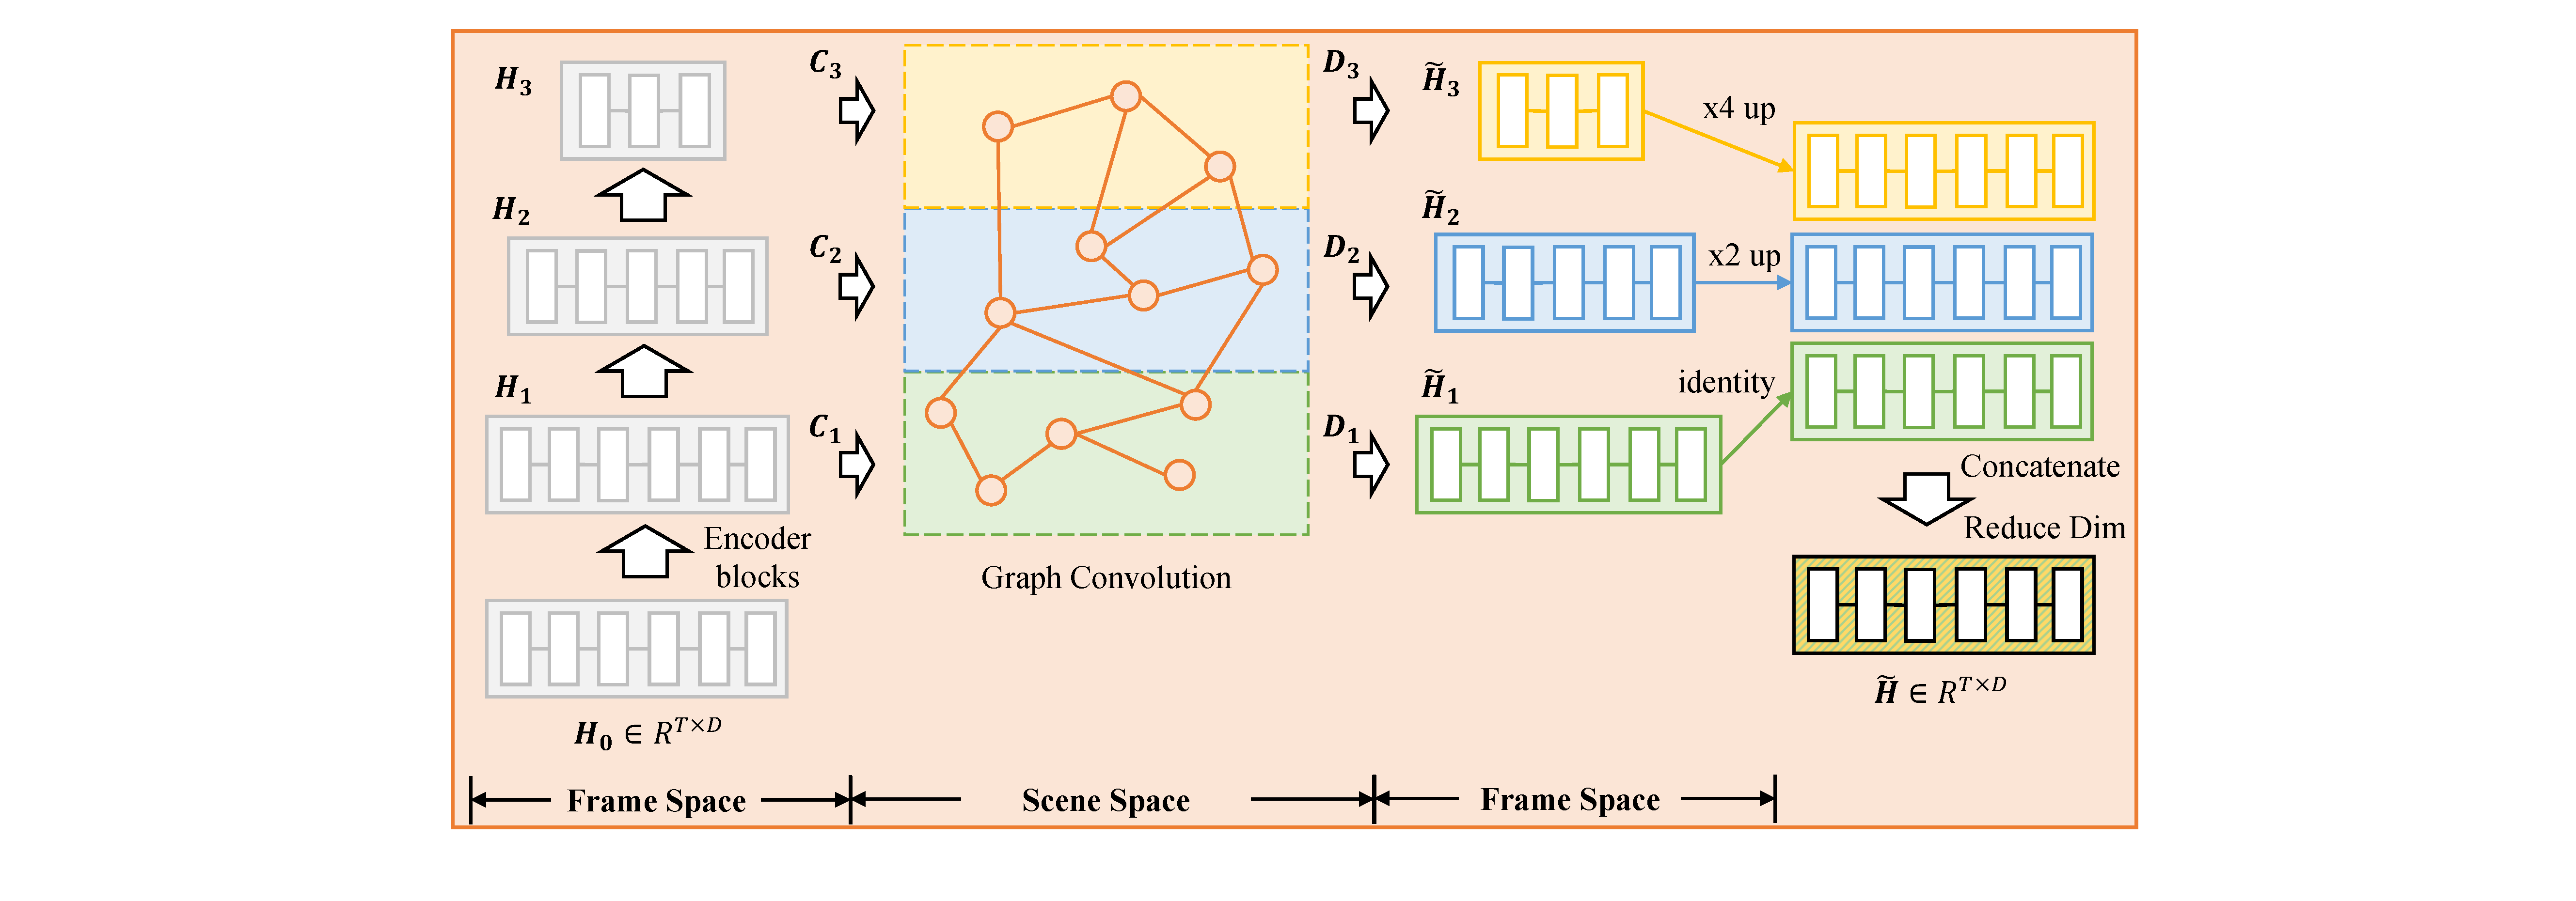
\includegraphics[width=0.95\linewidth]{chapter6/res/graph_fpn.pdf}
    \caption{图特征金字塔层}
    \label{ch6:fig:graph_fpn}
\end{figure}


\subsection{密集型头网络}

\begin{wrapfigure}{r}{0.3\linewidth}
    \centering
        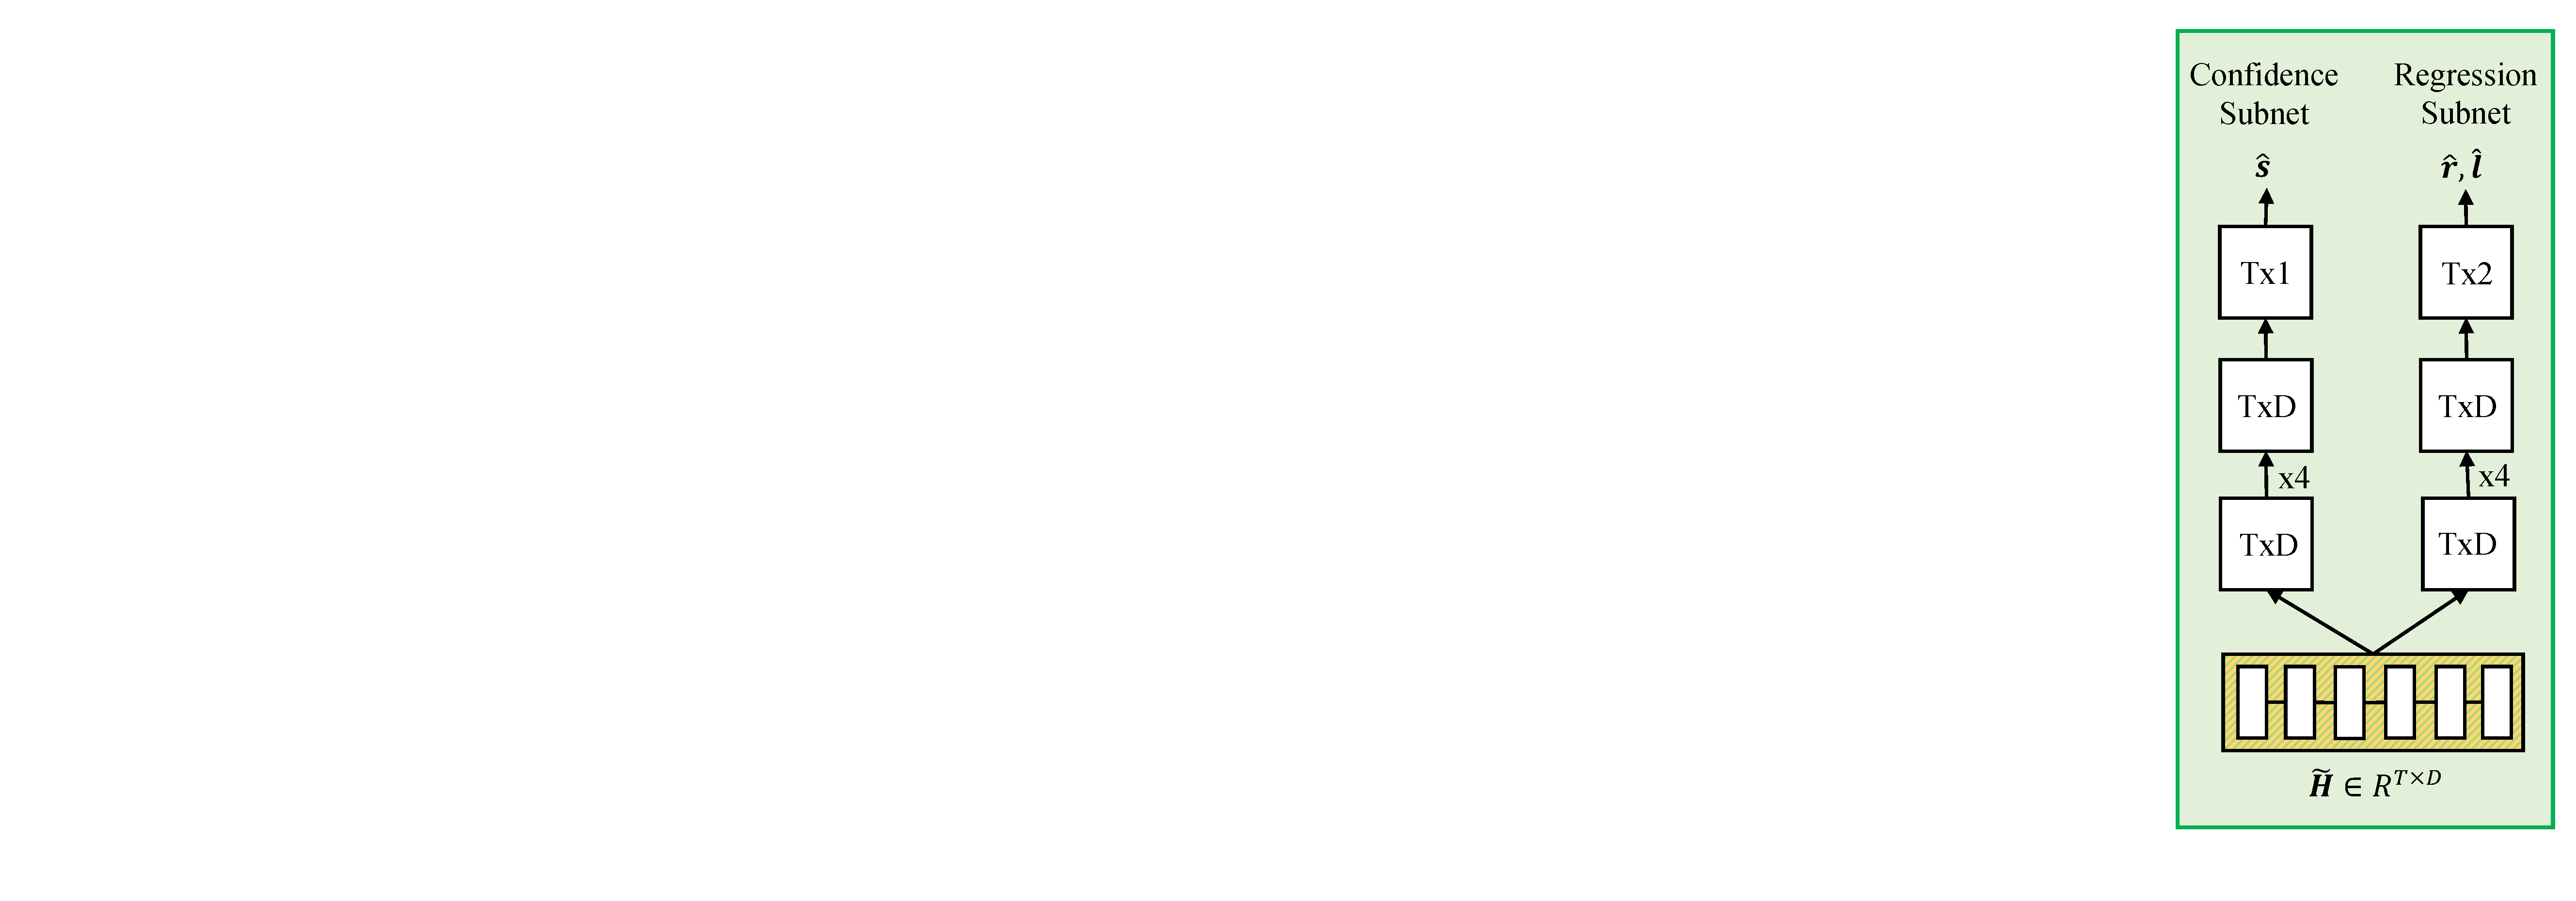
\includegraphics[width=0.9\linewidth]{chapter6/res/head_network.pdf}
    \captionof{figure}{密集型头网络}
    \label{ch3:fig:head_network}
\end{wrapfigure}

与目前的稀疏型自底向上模型不同,GDP将起始时刻到终止时刻间的每一帧都看成是正样本。对于每一帧,GDP包含两个分支网络(如图~\ref{ch3:fig:head_network}):

\textbf{回归分支}:对于每一帧,回归分支网络预测当前帧位置到两侧边界时刻的距离(起始时刻和终止时刻)。给定图特征金字塔层的输出$\tilde{\bm{H}}$,回归分支网络使用四个$D$通道的$1\times 3$的卷积层和一个1通道的$1\times 3$卷积层。最后用simoid激活函数预测左右的距离。我们只对正样本计算预测损失,对于第$i$帧,假设最终结果为($t_s, t_e$)(即:$t_s \leq i \leq t_e$),回归分支的目标为:
\begin{equation}
    l^*_i = i - t_s, \quad r^*_i = t_e - i,
\end{equation}
其中$l^*_i$和$r^*_i$分别表示第$i$帧到左右边界的距离。


\textbf{置信分支}:虽然每一帧都有独立的边界预测,但是不同帧预测边界的置信度往往不同。例如,离起始时刻比较近的帧预测起始时刻的置信度通常比终止时刻的置信度要高。基于这一观察,我们认为中心帧对两个边界预测的综合置信度最高。因此,我们将置信分支的目标设为:
\begin{equation}
s^*_i=\left\{
    \begin{aligned}
        & \frac{\min(l^*_i, r^*_i)}{\max(l^*_i, r^*_i)}, & t_s \leq i \leq t_e \\
        & 0.  & i < t_s ~\text{or}~ i > t_e \\
    \end{aligned}
    \right.
\end{equation}


\subsection{训练阶段和测试阶段}

\textbf{损失函数}:给定所有特征序列的预测$\{(\hat{t}_i, \hat{s}_i)\}^T_{i=1}$和相应的目标$\{(t^*_i, s^*_i)\}^T_{i=1}$,整个GDP的训练损失为:
\begin{equation}
    L = \frac{1}{T}L_{conf}(\hat{s}_i, s^*_i) + \frac{1}{T_p}\mathbf{1}_{\{s^*_i>0\}}L_{reg}(\hat{t}_i, t^*_i),
\end{equation}
其中$T$和$T_p$分别表示总样本和正样本的数量,$\mathbf{1}_{\{s^*_i>0\}}$是指示函数,当$s^*_i>0$时值为1,否则值为0。置信分支的分类损失$L_{conf}$为是二值化交叉熵,回归分支的回归损失$L_{reg}(\hat{t}_i, t^*_i) = L_{l1}(\hat{t}_i, t^*_i) + L_{IoU}(\hat{t}_i, t^*_i)$,其中$L_{l1}$是平滑的$l_1$损失函数,$L_{IoU}$是IoU损失函数(即:$-ln\frac{\min(\hat{r}_i, r^*_i)-\max(\hat{l}_i, l^*_i)}{\max(\hat{r}_i, r^*_i)-\min(\hat{l}_i, l^*_i)}$)。


\begin{figure}[tbp]
    \centering
    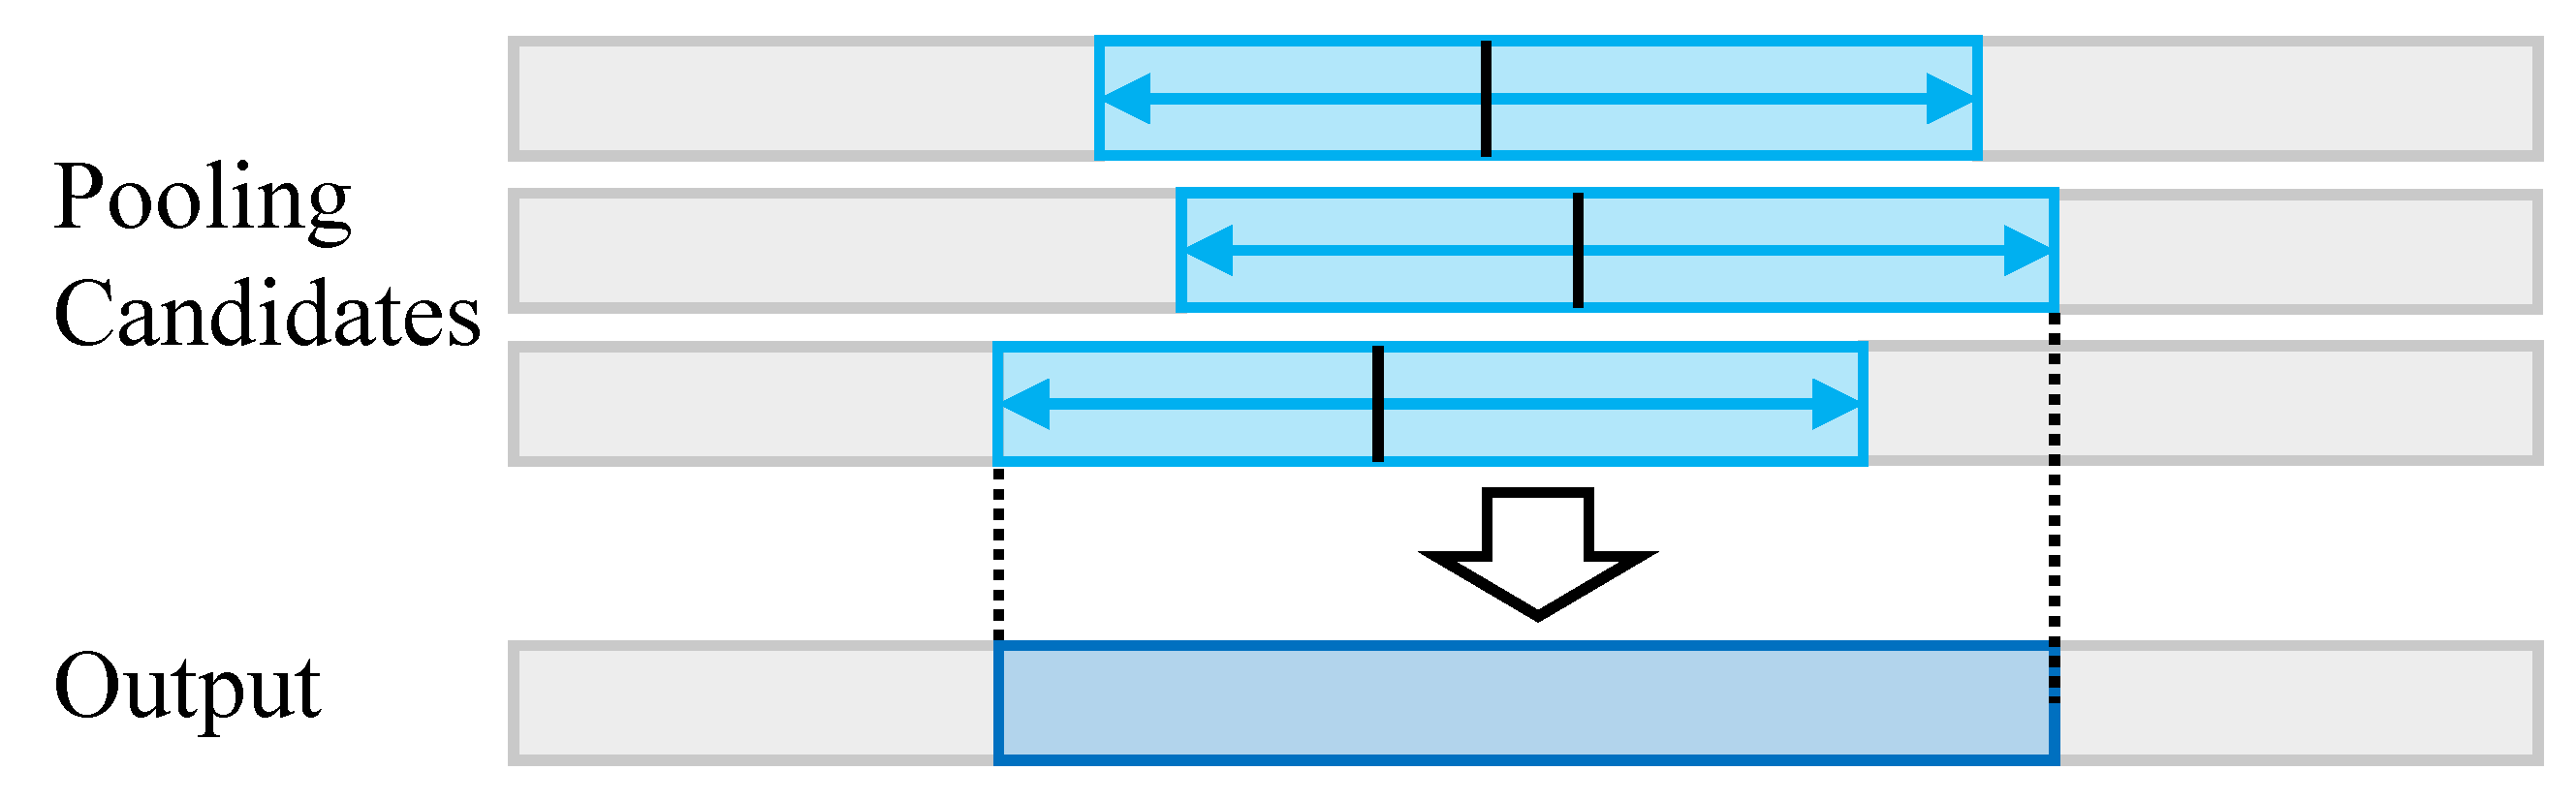
\includegraphics[width=0.7\linewidth]{chapter6/res/temporal_pooling.pdf}
    \caption{时域池化示意图}
    \label{ch6:fig:temporal_pooling}
\end{figure}


\textbf{测试阶段}:对于每一帧,我们可以得到单独的置信分数和边界预测。一种简单的方法就是直接选择置信分数最高的帧的边界预测作为最终结果,但是实验结果发现,这种方法容易造成预测结果存在较大的方差。为了缓解这种情况,我们使用一种简单的\textbf{时域池化}(Temporal Pooling)来融合多个预测结果。如图~\ref{ch6:fig:temporal_pooling}所示,我们使用候选帧的最左侧预测和最右侧预测分别作为最终的起始时刻和终止时刻预测。至于候选帧的选择,满足需要同时满足两个条件:(1)预测的视频片段和置信度最高的视频片段有重叠部分;(2)片段的置信度大于最高置信度乘以一个预先设定的阈值。


\section{实验设置与性能对比}

\subsection{视频片段检索数据集}

\noindent\textbf{\kaishu{基于语句的视频片段检索}}:我们在以下三个数据集上进行评估:

\noindent\textbf{TACoS}~\cite{regneri2013grounding}:它一共包含127个视频和17344个文本与视频序列对(样本)。我们参考现有的标准数据集划分~\cite{gao2017tall},将其中50\%的样本作为训练集,25\%的样本作为验证集,25\%的样本作为测试集。每个样本中视频的平均长度为5分钟。


\noindent\textbf{Charades-STA}~\cite{gao2017tall}:它一共包含12408个文本与视频序列对作为训练集,3720个文本与视频序列对作为测试集。每个样本中视频的平均长度为30秒。


\noindent\textbf{ActivityNet Captions}~\cite{krishna2017dense}:它是目前为止最大、最丰富的数据集,一共包含19209个视频。我们参考现有的工作~\cite{yuan2019find}, 使用37421个文本与视频序列作为训练集,17505个文本与视频序列作为测试集。每个样本中视频的平均长度为2分钟。


\noindent\textbf{\kaishu{基于视频的视频片段检索}}:我们在以下数据集上进行评估:

\noindent\textbf{ActivityNet-VRL}~\cite{feng2018video}:它是目前唯一公开发布的数据集。它对动作识别数据集ActivityNet~\cite{caba2015activitynet}共200个类别的视频进行了重组,其中任意选取160个类别对应的视频作为训练集,20个类别对应的视频作为验证集,以及剩余20个类别对应的视频作为测试集。这种零样本式的数据集划分能够评估模型的泛化能力。在训练阶段,查询视频和引用视频是随机选取的。在测试阶段,查询视频和引用视频是固定的。

\subsection{评价指标}


\noindent\textbf{\kaishu{基于语句的视频片段检索}}:我们参考现有工作,使用下列两种通用的评价指标:

\noindent\textbf{R@N, IoU@$\theta$}:在测试集中,每个样本预测分数最高的n个的结果重叠度(Intersection-over-Union,IoU)大于$\theta$的百分比。由于自底向上框架的特性,我们仅考虑$N=1$。

\noindent\textbf{mIoU}:测试集中所有测试样本的平均的重叠度。


\noindent\textbf{\kaishu{基于视频的视频片段检索}}:我们使用以下评价指标:

\noindent\textbf{mAP@1}:在不同阈值下最高预测结果的平均精度均值(mAP)。


\subsection{实验设定}
给定一个视频序列$\mathcal{V}$,我们首先对视频进行下采样,用Sports-1M数据集~\cite{karpathy2014large}预训练的网络提取C3D特征~\cite{tran2015learning},然后利用PCA将特征维度降低到500维作为初始的视频特征。当查询为自然语句时,我们先将语句的最大长度设为15,然后每个单词用300维的Glove向量~\cite{pennington2014glove}作为初始的编码,然后利用一个可学习的映射矩阵将维度也映射到500维。当查询为视频片段时,我们使用和之前参考视频同样的预处理。中间所有层的维度都设为128,节点数$N_1$、$N_2$和$N_3$分别设为10。这个网络利用Adam~\cite{kingma2015adam}对模型进行优化,整个模型训练100个数据集周期,初始的学习率设为0.0001,训练的批量大小设为16。


\subsection{视频片段检索性能对比}

\textbf{基于语句查询的视频片段检索}

%%%%%%%%%%%%%%%%%%% SOTA NLVL %%%%%%%%%%%%%%%%%%%%%%%

\begin{table*}[tbp]
    \centering
    \scalebox{0.75}{
        \begin{tabular}{|l|l| c c c| c c c | c c c |}
            \hline
            & \multirow{2}{*}{Method} & \multicolumn{3}{c|}{TACoS} & \multicolumn{3}{c|}{Charades-STA} & \multicolumn{3}{c|}{ActivityNet Captions} \\
            & & IoU@0.1 & IoU@0.3 & mIoU & IoU@0.3 & IoU@0.5 & IoU@0.7 & IoU@0.3 & IoU@0.5 & mIoU  \\
            \hline
            \parbox[t]{2mm}{\multirow{10}{*}{\rotatebox[origin=c]{90}{TD}}} & VSA-RNN & 8.84 & 6.91 & - & - & 10.50 & 4.32 & - & - & - \\
            & VSA-STV & 15.01 & 10.77 & - & - & 16.91 & 5.81 & - & - & - \\
            & CTRL & 24.32 & 18.32 & - & - & 23.63 & 8.89 & - & - & - \\
            & ROLE & - & - & - & 25.26 & 12.12 & - & - & - & - \\
            & ACRN & 24.22 & 19.52 & - & - & - & - & - & - & - \\
            & MCF & 25.84 & 18.64 & - & - & - & - & - & - & - \\
            & TGN & - & - & - & - & - & - & 43.81 & 27.93 & - \\
            & ACL & 28.31 & 22.07 & - & - & 26.47 & 11.23 & - & - & - \\
            & SAP & 31.15 & - & - & - & 27.42 & 13.36 & - & - & - \\
            & QSPN & - & - & - & \textbf{54.70} & 35.60 & 15.80 & 45.30 & 27.70 & - \\
            \cline{1-2}
            \parbox[t]{2mm}{\multirow{2}{*}{\rotatebox[origin=c]{90}{RL}}} & RWM & - & - & - & - & 36.70 & - & - & 36.90 & - \\
            & SM-RL & 26.51 & 20.25 & - & - & 24.36 & 11.17 & - & - & - \\
            \cline{1-2}
            \parbox[t]{2mm}{\multirow{4}{*}{\rotatebox[origin=c]{90}{BU}}} & L-NET & - & - & 13.41 & - & - & - & - & - & - \\
            & ABLR-aw & 31.60 & 18.90 & 12.50 & - & - & - & 53.65 & 34.91 & 35.72 \\
            & ABLR-af & 34.70 & 19.50 & 13.40 & - & - & - & 55.67 & 36.79 & 36.99 \\
            & \textbf{GDP} & \textbf{39.68} & \textbf{24.14} & \textbf{16.18} & 54.54 & \textbf{39.47} & \textbf{18.49} & \textbf{56.17} & \textbf{39.27} & \textbf{39.80} \\
            \hline
        \end{tabular}
    }
    \caption{不同基于语句查询的视频片段检索方法的性能对比}
    \label{ch6:tab:sota_nlvl}
\end{table*}


\textbf{基于视频查询的视频片段检索}


%%%%%%%%%%%%%%%%%%%%% SOTA VRL %%%%%%%%%%%%%%%%%%%%%%%
\begin{table}[tbp]
    \centering
    \scalebox{0.9}{
        \begin{tabular}{|l| c c c c c c |}
            \hline
            mAP@1 & 0.5 & 0.6 & 0.7 & 0.8 & 0.9 & Avg   \\
            \hline
            Frame-level  & 18.8 & 13.9 & 9.6 & 5.0 & 2.3 & 9.9 \\
            Video-level & 24.3 & 17.4 & 12.0 & 5.9 & 2.2 & 12.4 \\
            SST & 33.2  & 24.7 & 17.2 & 7.8 & 2.7 & 17.1  \\
            CGBM & 43.5 & 35.1 & 27.3 & 16.2 & 6.5 & 25.7 \\
            \textbf{GDP} & \textbf{44.0} & \textbf{35.4} & \textbf{27.7} & \textbf{20.0} & \textbf{12.1} & \textbf{27.8} \\
            \hline
        \end{tabular}
    }
    \caption{不同基于视频查询的视频片段检索方法的性能对比}
    \label{ch6:tab:sota_vrl}
\end{table}


\begin{figure}[tbp]
    \centering
    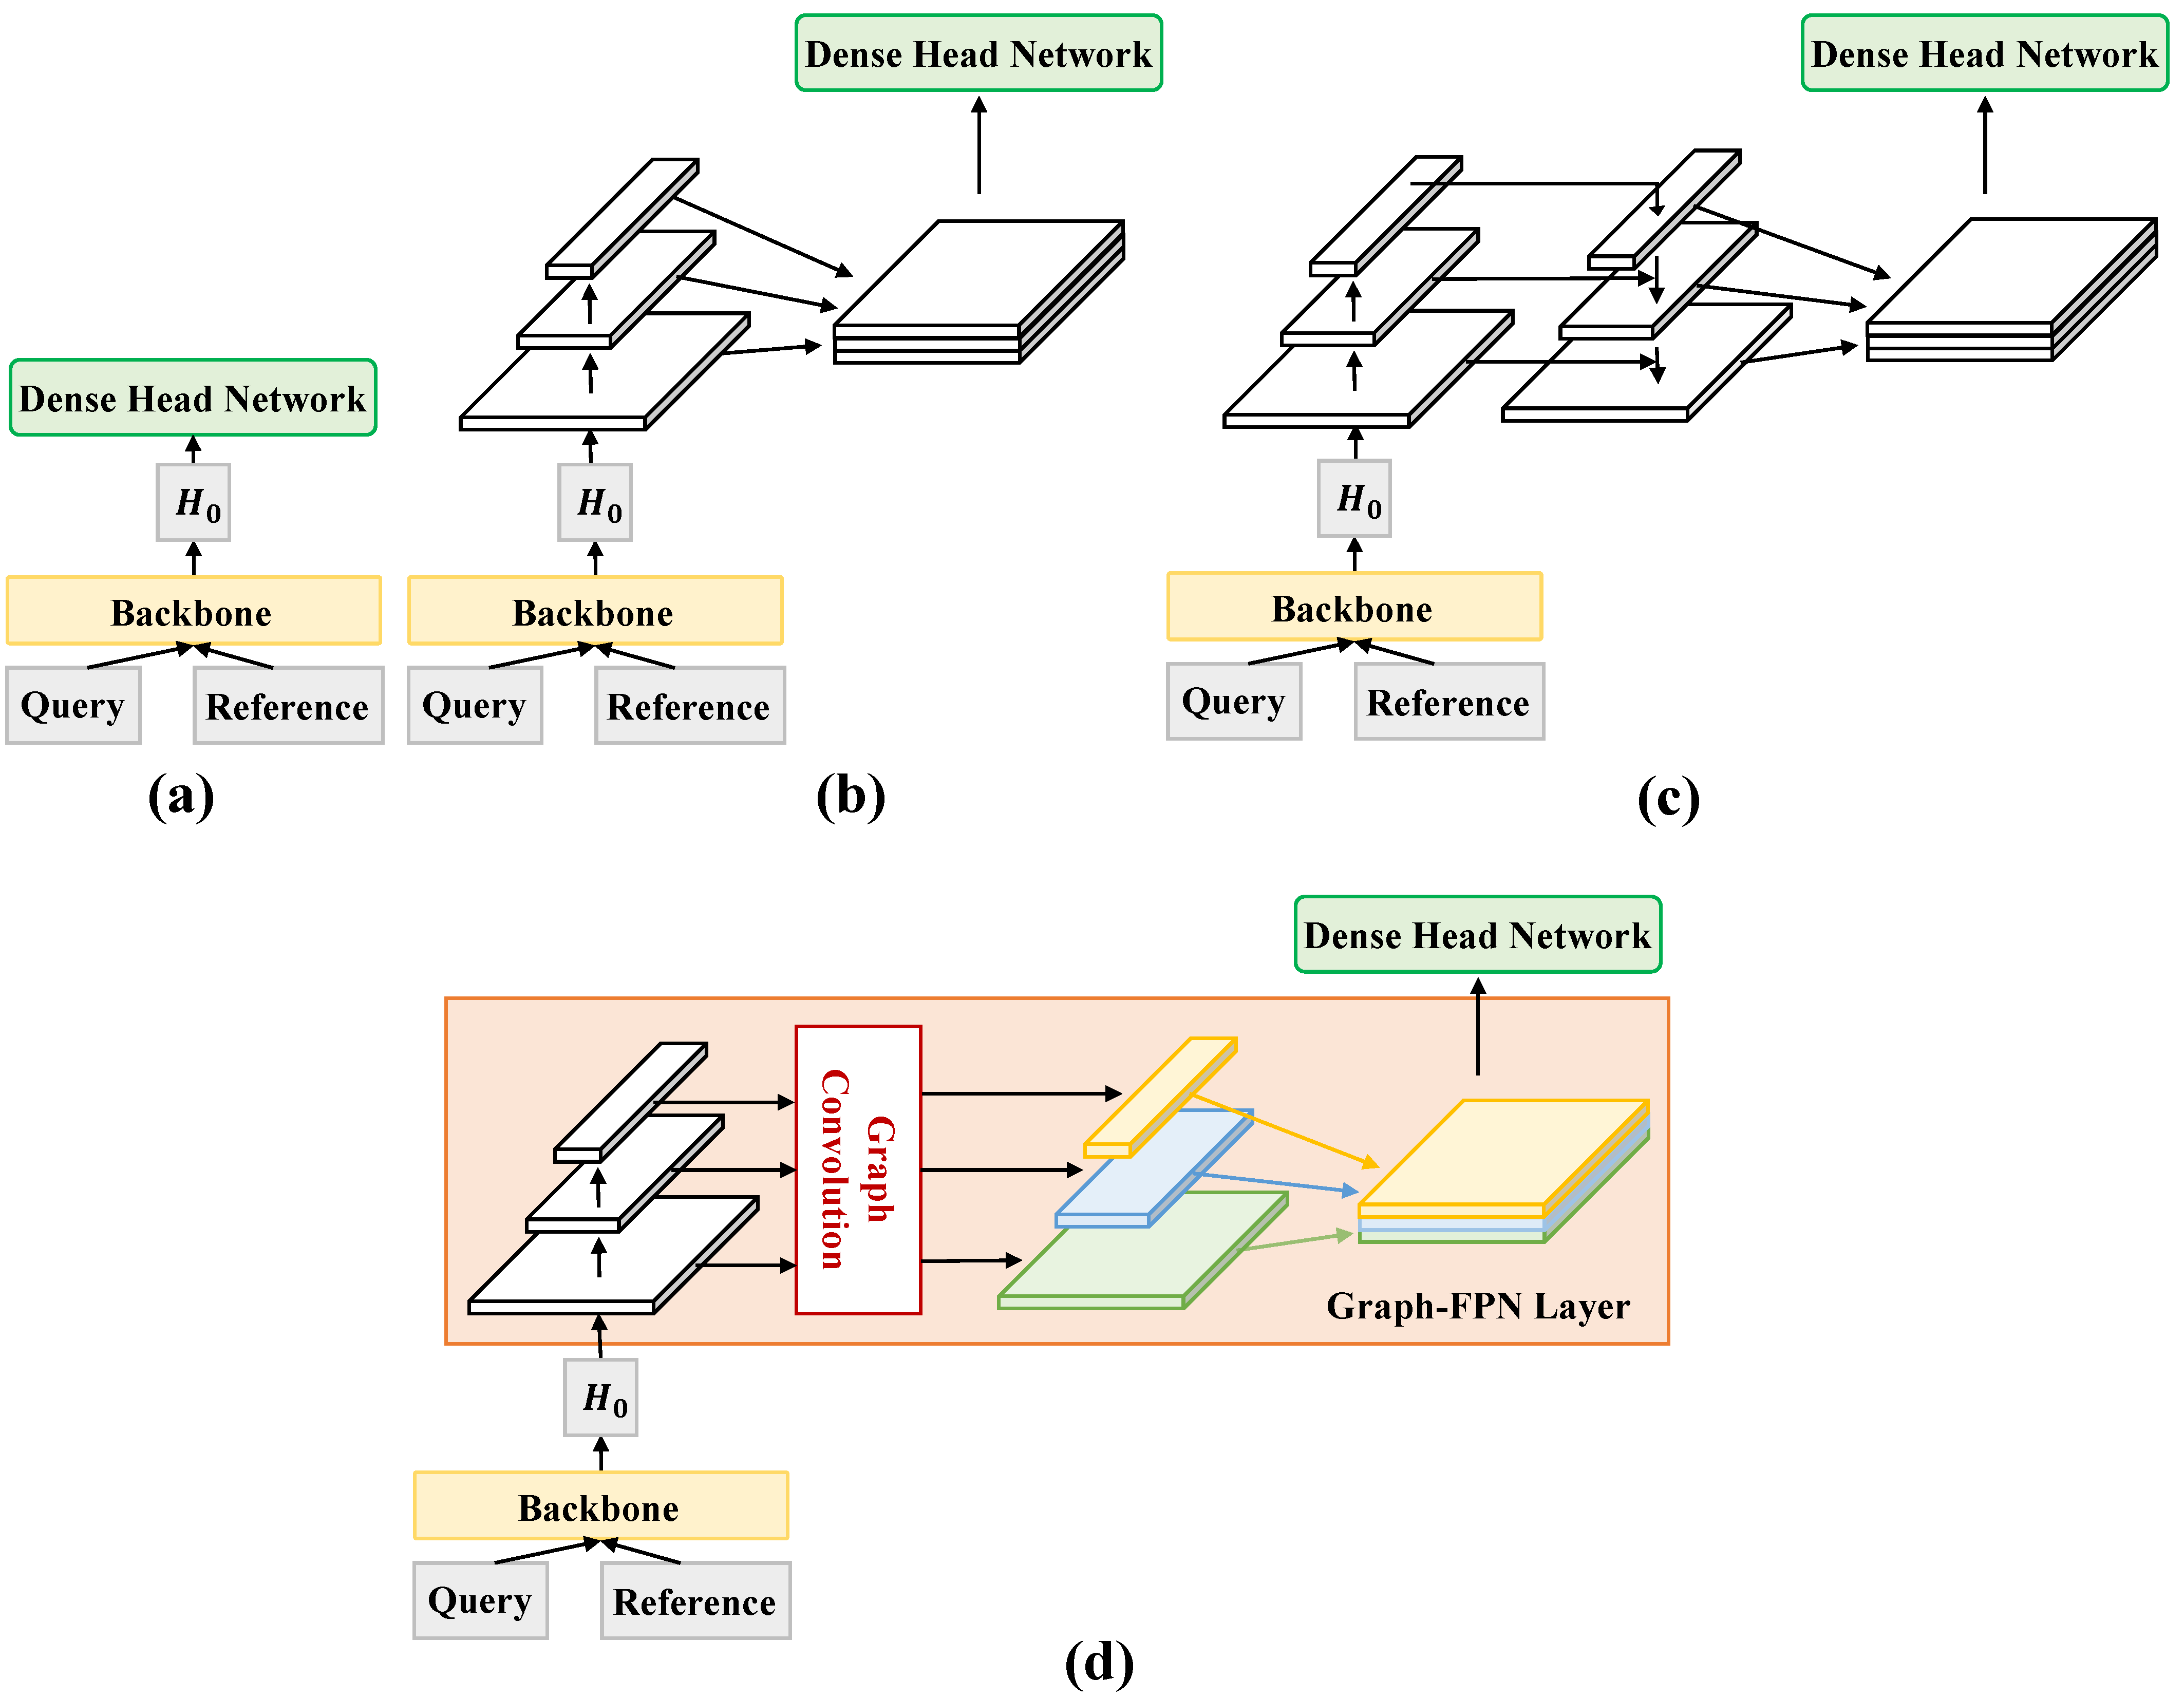
\includegraphics[width=0.9\linewidth]{chapter6/res/ablative_backbone.pdf}
    \caption{同一骨干网络不同特征优化层的性能对比}
    \label{ch6:fig:ablative_backbone}
\end{figure}


%%%%%%%%%%%%%%%%%%% Ablation about Backbone NLVL %%%%%%%%%%%%%%%%
\begin{table*}[htbp]
    \centering
    \scalebox{0.9}{
        \begin{tabular}{|c | c c c c| c c c c| c c c c|}
            \hline
            & \multicolumn{4}{c|}{TACoS} & \multicolumn{4}{c|}{Charades-STA} & \multicolumn{4}{c|}{ActivityNet Captions}  \\
            \hline
            \multirow{2}{*}{Model} & \multicolumn{3}{c|}{IoU@} & \multirow{2}{*}{mIoU} & \multicolumn{3}{c|}{IoU@} & \multirow{2}{*}{mIoU} & \multicolumn{3}{c|}{IoU@} & \multirow{2}{*}{mIoU} \\
            & 0.1 & 0.3 & 0.5 & \multicolumn{1}{|c|}{} & 0.3 & 0.5 & 0.7 & \multicolumn{1}{|c|}{}  & 01. & 0.3 & 0.5 & \multicolumn{1}{|c|}{} \\
            \hline
            A & 37.4 & 23.3 & 11.5 & 15.3 & 51.8 & 38.3 & 17.8 & 35.1 & 72.1 & 56.0 & \textbf{40.7} & 39.3  \\
            B & 37.3 & 23.1 & \textbf{13.9} & 15.8 & 53.8 & 38.6 & 18.4 & 36.0 & 73.1 & 56.2 & 40.3 & 39.5  \\
            C & 36.8 & 23.1 & 13.8 & 15.7  & 52.6 & 38.9 & 18.3 & 35.8 & 73.7 & 54.7 & 38.9 & 39.4 \\
            D & \textbf{39.7} & \textbf{24.1} & 13.5 & \textbf{16.2} & \textbf{54.5} & \textbf{39.5} & \textbf{18.5} & \textbf{36.6} & \textbf{75.0} & \textbf{56.2} & 39.3 & \textbf{39.8} \\
            \hline
        \end{tabular}
    }       
    \caption{基于语句查询的视频片段检索任务中模型A、B、C、D的性能对比}
    \label{ch6:tab:nlvl_ablation_backbone}
\end{table*}


%%%%%%%%%%%%%%%%%%% Ablation about Backbone VRL %%%%%%%%%%%%%%%%
\begin{table*}[htbp]
    \centering
    \scalebox{0.9}{
        \begin{tabular}{|c |c c c c c|}
            \hline
            mAP@1 & 0.5 & 0.6 & 0.7 & 0.8 & 0.9 \\
            \hline
            A & 41.1 & 34.2 & 27.7  & \textbf{20.3} & 6.8 \\
            B & 43.3 & 35.0 & \textbf{27.9} & 18.2  & 9.6 \\
            C & 42.9 & 34.5 & 26.9 & 18.8  & 8.4 \\
            D & \textbf{44.0} & \textbf{35.4} & 27.7 & 20.0 & \textbf{12.1} \\
            \hline
        \end{tabular}
    }       
    \caption{基于视频查询的视频片段检索任务中模型A、B、C、D的性能对比}
    \label{ch6:tab:vrl_ablation_backbone}
\end{table*}


%%%%%%%%%%%%%%%% Ablation Head Network %%%%%%%%%%%%%%
\begin{table}[tbp]
    \centering
    \scalebox{0.85}{
        \begin{tabular}{|l|l|l| c c c|}
            \hline
            & \multirow{2}{*}{Dataset} & \multirow{2}{*}{Metric} & \multicolumn{3}{c|}{Head Network} \\
            &  &  & Sparse & Dense$^*$ & Dense \\
            \hline
            \parbox[t]{2mm}{\multirow{12}{*}{\rotatebox[origin=c]{90}{NLVL}}} &\multirow{4}{*}{TACoS} & IoU@0.1 & 32.3 & 36.5 & \textbf{39.7} \\
            & & IoU@0.3 & 18.7 & 22.9 & \textbf{24.1}  \\
            & & IoU@0.5 & 9.6 & 13.0 & \textbf{13.5}  \\
            & & mIoU & 12.9 & 15.2 & \textbf{16.2}  \\
            \cline{2-6}
            & \multirow{4}{*}{Charades-STA} & IoU@0.3 & 52.9 & 53.9 & \textbf{54.5} \\
            & & IoU@0.5 & 31.4 & 39.0 & \textbf{39.5}   \\
            & & IoU@0.7 & 14.7 & 18.3 & \textbf{18.5} \\
            & & mIoU & 35.1 & 36.1 & \textbf{36.6}  \\
            \cline{2-6}
            & \multirow{4}{*}{ActivityNet} & IoU@0.1 & 72.4 & 73.5 & \textbf{75.0}  \\
            & & IoU@0.3 & 53.0 & 55.9 & \textbf{56.2} \\
            & & IoU@0.5 & 37.5 & \textbf{39.8} & 39.3  \\
            & & mIoU & 39.0 & 39.3 & \textbf{39.8}  \\
            \hline
            \parbox[t]{2mm}{\multirow{6}{*}{\rotatebox[origin=c]{90}{VRL}}} &\multirow{6}{*}{ActivityNet} & tIoU@0.5 & 41.6 & 42.3 & \textbf{44.0}  \\
            & & tIoU@0.6 & 30.5 & 35.3 & \textbf{35.4}   \\
            & & tIoU@0.7 & 25.7 & 27.6 & \textbf{27.7} \\
            & & tIoU@0.8 & 19.8 & \textbf{20.6} & 20.0 \\
            & & tIoU@0.9 & 8.5 & \textbf{12.5} & 12.1 \\
            & & Average & 25.2 & 27.7 & \textbf{27.8}  \\
            \hline
        \end{tabular}
    }
    \caption{密集型头网络和稀疏型头网络对比}
    \label{ch6:tab:ablation_head}
\end{table}


\begin{figure}[tbp]
    \centering
    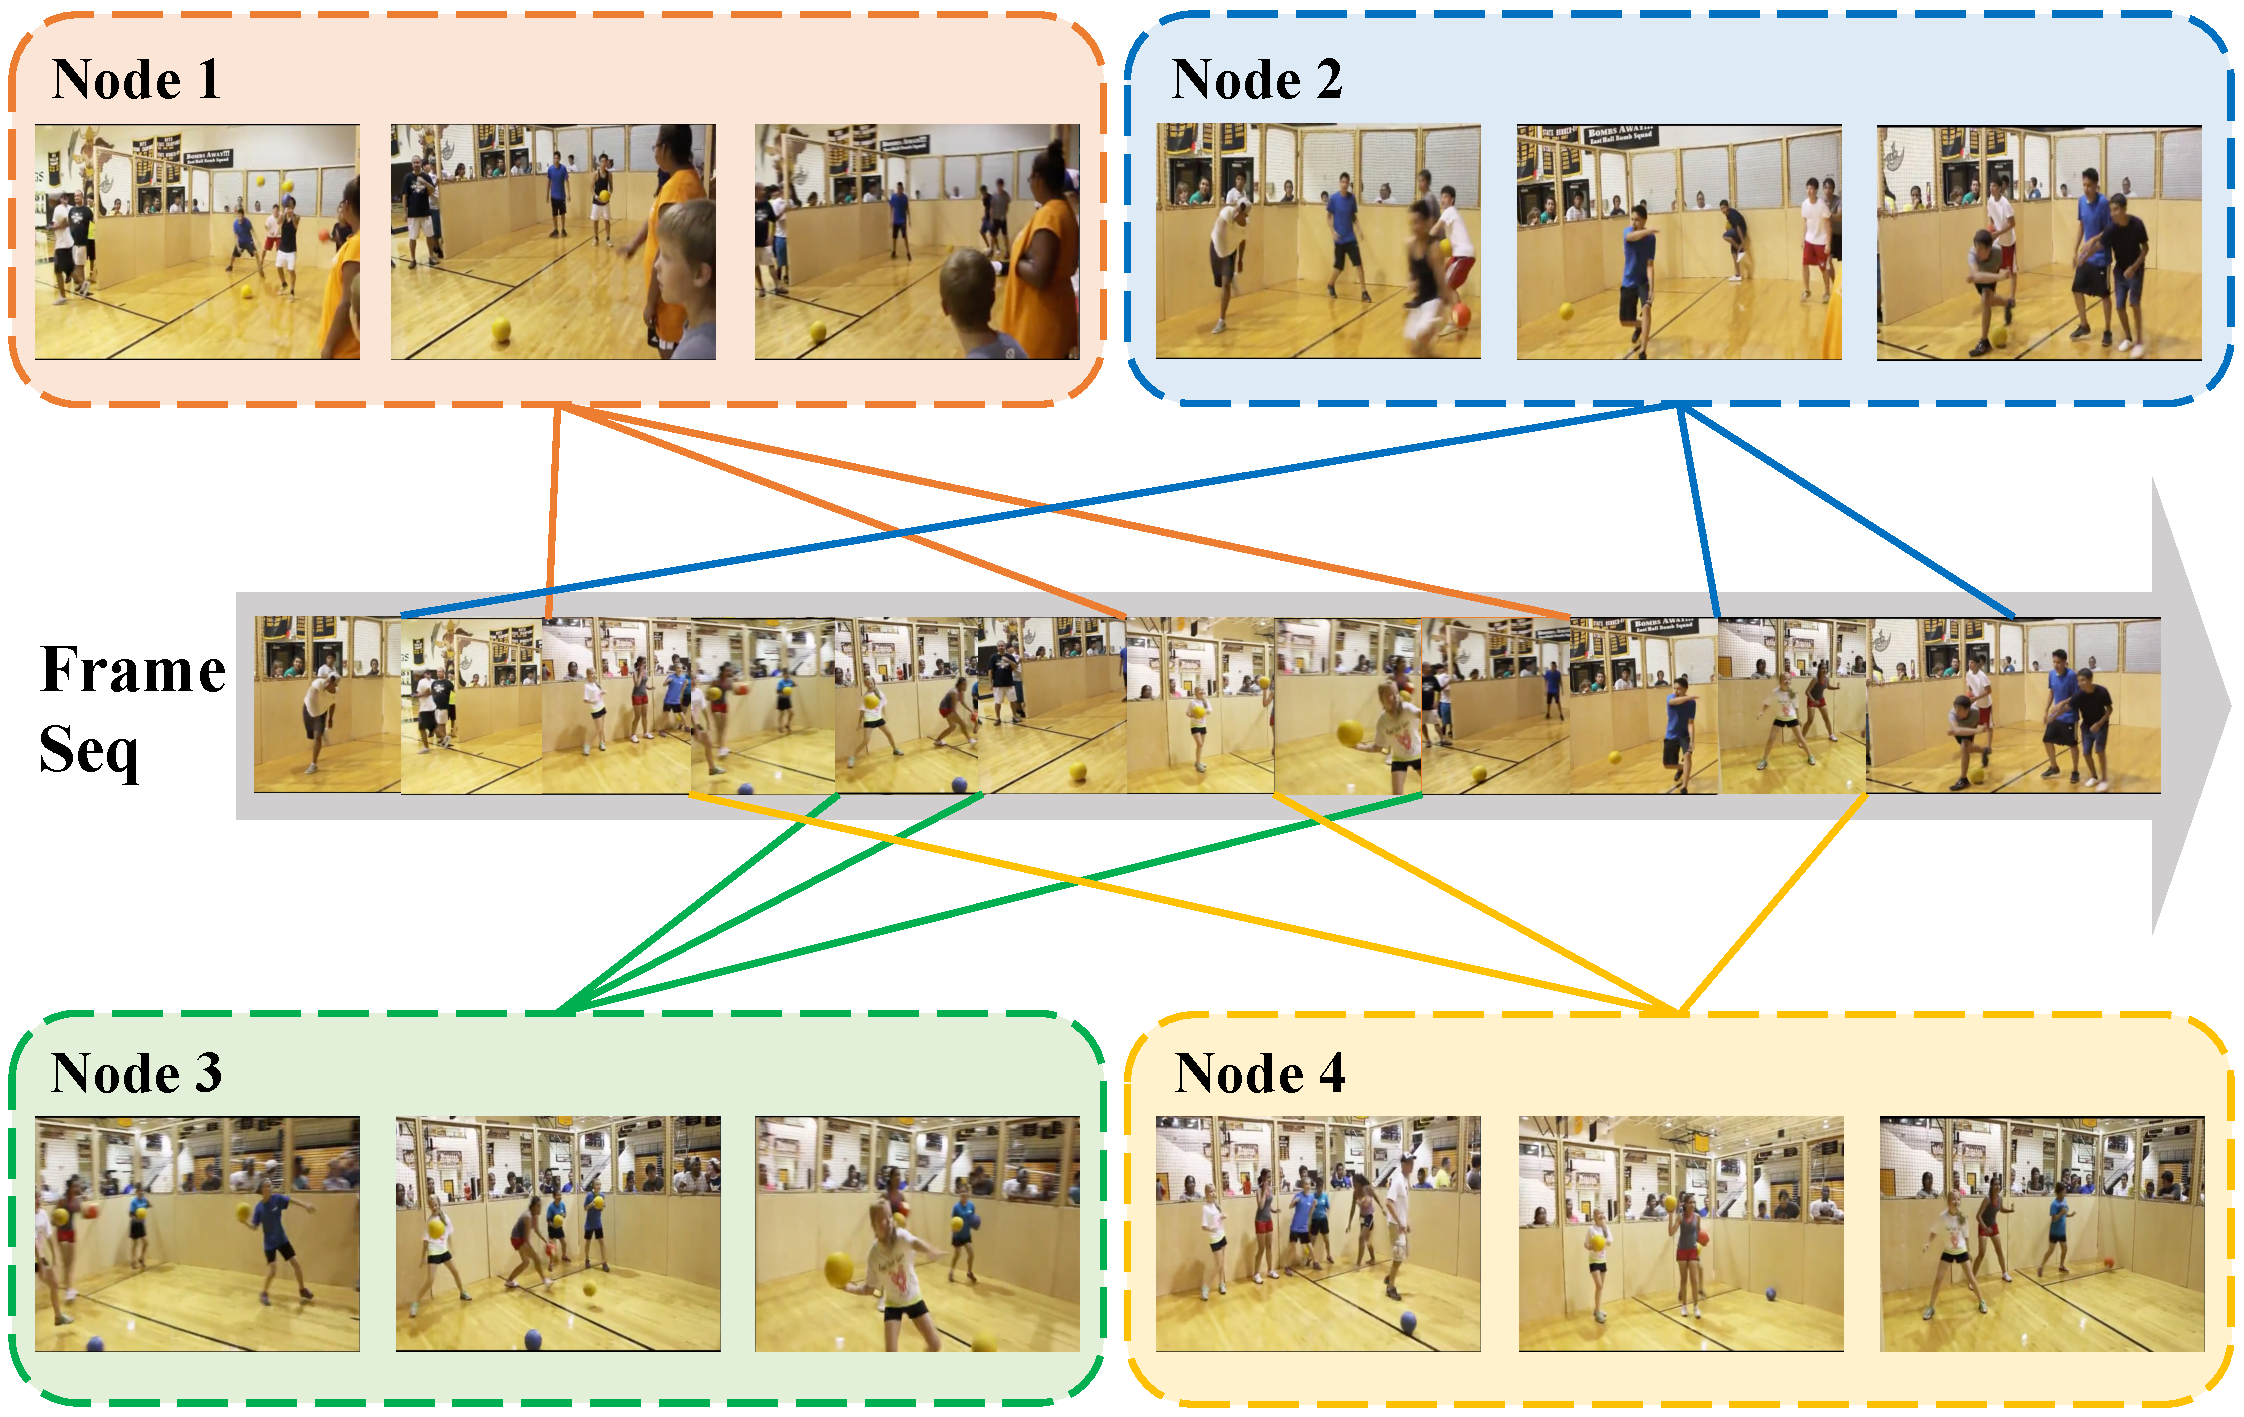
\includegraphics[width=0.8\linewidth]{chapter6/res/node_visualization.pdf}
    \caption{场景空间中的节点可视化}
    \label{ch6:fig:node_visualization}
\end{figure}

\section{本章小结}

